\chapter[Операторы управления]{Операторы управления}

В этой главе описаны основные операторы языка \Sys{C++}: условный оператор \Sys{if}, оператор выбора
\Sys{switch}, операторы цикла \Sys{while}, \Sys{do}…\Sys{while} и
\Sys{for}. Изложена методика составления алгоритмов с помощью блок-схем. Приводится большое количество
примеров составления программ различной сложности. 

\section[Основные конструкции алгоритма]{Основные конструкции алгоритма}
При разработке простейших программ несложно перейти от словесного описания к написанию программы. Однако большинство
реально разрабатываемых программ довольно сложные и созданию программы предшествует разработка алгоритма\footnote{От
\emph{algorithmi}, \emph{algorismus}, первоначально латинская транслитерация имени математика
аль-Хорезми.}. \index{Алгоритм}\emph{Алгоритм} --- это чёткое описание последовательности действий, которые
необходимо выполнить, для того чтобы при соответствующих исходных данных получить требуемый результат. Одним из
способов представления алгоритма является \index{Блок-схема}\emph{блок-схема}. При составлении блок-схемы
все этапы решения задачи изображаются с помощью различных геометрических фигур. Эти фигуры называют блоками и, как
правило, сопровождают надписями. Последовательность выполнения этапов указывают при помощи стрелок, соединяющих эти
блоки. Типичные этапы решения задачи изображаются следующими геометрическими фигурами:
\begin{itemize}
\item блок начала-конца (рис. \ref{ch03:refDrawing0}). Надпись внутри блока: «начало» («конец»);

\item блок ввода-вывода данных (рис. \ref{ch03:refDrawing1}). Надпись внутри блока: ввод (вывод или печать) и список вводимых
(выводимых) переменных;

\item блок решения или арифметический (рис. \ref{ch03:refDrawing2}). 
Внутри блока записывается действие, вычислительная операция
или группа операций;

\item условный блок (рис. \ref{ch03:refDrawing3}). Логическое условие записывается внутри блока. В результате проверки условия
осуществляется выбор одного из возможных путей (ветвей) вычислительного процесса. 
\end{itemize}
{\footnotesize
%{\renewcommand{\captiontitlefont}{\footnotesize\sffamily}
   \floatsetup[widefloat]{margins=hangleft,labelfont=footnotesize}
   \begin{figure}%
   \begin{floatrow}[4]
   %\captionnamefont{\footnotesize}
   \ffigbox[\FBwidth]
   {%\captionnamefont{\footnotesize}
   \captionsetup{labelfont=footnotesize}\caption{\footnotesize Блок начала-конца алгоритма}%
   \label{ch03:refDrawing0}}
   {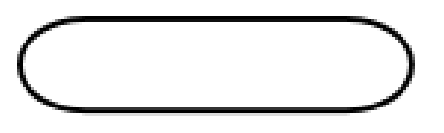
\includegraphics[width=0.18\textwidth,keepaspectratio]{img/ris_3_1}}%\hspace*{0.01\textwidth}

   \ffigbox[\FBwidth]
   {\caption{\footnotesize Блок ввода-вывода данных}%
   \label{ch03:refDrawing1}}
   {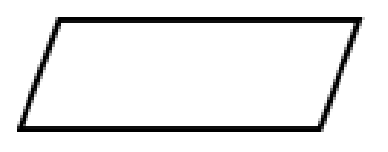
\includegraphics[width=0.18\textwidth,keepaspectratio]{img/ris_3_2}}%\hspace*{0.01\textwidth}

   %\ffigbox[\Xhsize/2]
   \ffigbox[\FBwidth]%[\FBheight][t]
   {\caption{\footnotesize Арифмети\-чёс\-кий блок}%
   \label{ch03:refDrawing2}}
   %{{\setlength\unitlength{\hsize/58}%^^A
   {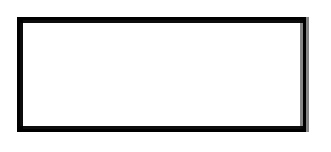
\includegraphics[width=0.18\textwidth,keepaspectratio]{img/ris_3_3}}%\hspace*{0.01\textwidth}
   %}}}
   %\ffigbox[\Xhsize]
   \ffigbox[\FBwidth]%[\FBheight][t]
   {\caption{\footnotesize Условный блок}%
   \label{ch03:refDrawing3}}
   {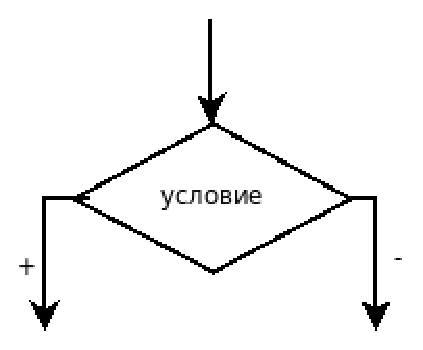
\includegraphics[width=0.31\textwidth,keepaspectratio]{img/ris_3_4}}%}
   \end{floatrow}
   \end{figure}%
}

Рассмотренные блоки позволяют описать три \index{Алгоритм!основные конструкции}\emph{основные конструкции
алгоритма}: линейный процесс, разветвляющийся процесс и циклический процесс.

\index{Алгоритм!линейный}\emph{Линейный процесс} это конструкция, представляющая собой последовательное
выполнение двух или более операторов (рис.~\ref{ch03:refDrawing4}).
\index{Алгоритм!разветвляющийся}\emph{Разветвляющийся процесс} задаёт выполнение одного или другого
оператора в зависимости от выполнения условия (рис.~\ref{ch03:refDrawing5}).
\index{Алгоритм!циклический}\emph{Циклический процесс} задаёт многократное выполнение оператора или группы
операторов (рис.~\ref{ch03:refDrawing6}).

{\footnotesize
%{\renewcommand{\captionnamefont}{\footnotesize\sffamily}
   \floatsetup[widefloat]{margins=hangleft}
   \begin{figure}%
   \begin{floatrow}[3]
   \captionnamefont{\footnotesize}
   \ffigbox[\FBwidth]
   {\captionnamefont{\footnotesize}\caption{\footnotesize Ли\-ней\-ный процесс}%
   \label{ch03:refDrawing4}}
   {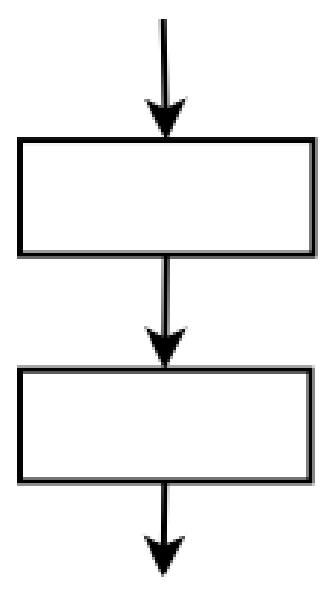
\includegraphics[width=0.18\textwidth,keepaspectratio]{img/ris_3_5}}%\hspace*{0.01\textwidth}

   %\ffigbox[\Xhsize/2]
   \ffigbox[\FBwidth]%[\FBheight][t]
   {\caption{\footnotesize Разветвляющийся процесс}%
   \label{ch03:refDrawing5}}
   %{{\setlength\unitlength{\hsize/58}%^^A
   {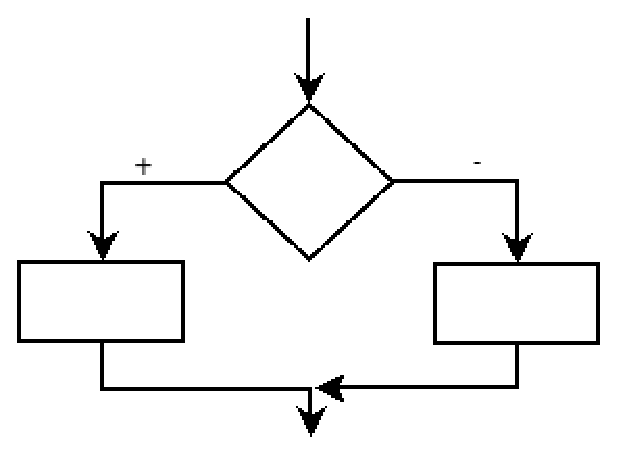
\includegraphics[width=0.42\textwidth,keepaspectratio]{img/ris_3_6}}%\hspace*{0.01\textwidth}
   %}}}
   %\ffigbox[\Xhsize]
   \ffigbox[\FBwidth]%[\FBheight][t]
   {\caption{\footnotesize Циклический процесс}%
   \label{ch03:refDrawing6}}
   {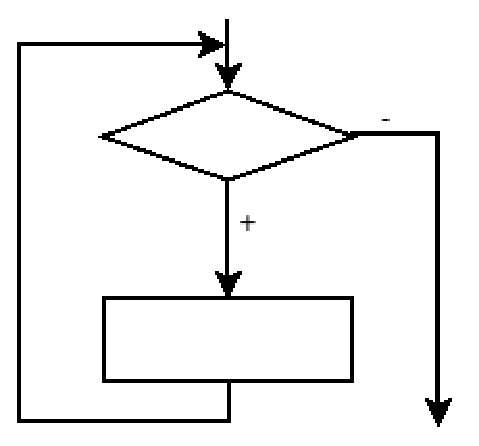
\includegraphics[width=0.32\textwidth,keepaspectratio]{img/ris_3_7}}%}
   \end{floatrow}
   \end{figure}%
%\renewcommand{\captionnamefont}{\small\sffamily}
}

Нетрудно заметить, что каждая из основных конструкций алгоритма имеет один вход и один выход. Это позволяет вкладывать
конструкции друг в друга произвольным образом и составлять алгоритмы для решения задач любой сложности.

Одним из важных понятий при написании программ на \Sys{С}(\Sys{С++}) является понятие составного оператора.

\section[Составной оператор]{Составной оператор}
\index{Оператор!составной}\emph{Составной оператор} --- это группа операторов, отделённых друг от друга
точкой с запятой, начинающихся с открывающей фигурной скобки \{ и заканчивающихся закрывающейся
фигурной скобкой \}:
\begin{lstlisting}
{
  `\Sys{оператор\_1;}`
  `\Sys{...}`
  `\Sys{оператор\_n;}`
}
\end{lstlisting}

Транслятор воспринимает составной оператор как одно целое.

Рассмотрим операторы языка \Sys{С++}, реализующие основные конструкции алгоритма.

\section[Условные операторы]{Условные операторы}
Одна из основных конструкций алгоритма --- 
\index{Оператор!разветвляющийся}\emph{разветвляющийся процесс}. Он реализован в языке
\Sys{С++} двумя условными операторами: \Sys{if} и \Sys{switch}. Рассмотрим каждый из них.

\subsection[Условный оператор]{Условный оператор}
При решении большинства задач порядок вычислений зависит от определённых условий, например, от исходных данных или от
промежуточных результатов, полученных на предыдущих шагах программы. Для организации вычислений в зависимости от
какого-либо условия в \Sys{С++} предусмотрен \index{Оператор!условный}\emph{условный оператор} \Sys{if}, 
который в общем виде записывается следующим образом:
\begin{lstlisting}
if `\Sys{(условие) оператор\_1}`; else `\Sys{оператор\_2}`;
\end{lstlisting}
где \Sys{условие} --- это логическое (или целое) выражение, переменная или константа, 
\Sys{оператор\_1} и \Sys{оператор\_2} --- любой оператор языка \Sys{С(С++)}.

Работает условный оператор следующим образом. Сначала вычисляется значение выражения, указанного в скобках. Если
оно не равно нулю, т.е. имеет значение истина (\Sys{true}), выполняется \Sys{оператор\_1}. В
противном случае, когда выражение равно нулю, т.е. имеет значение ложь (\Sys{false}), выполняется
\Sys{оператор\_2}. Алгоритм, который реализован в условном операторе \Sys{if}, представлен на
рис.~\ref{ch03:refDrawing7}.

%\begin{figure}[htb]
%\begin{center}
%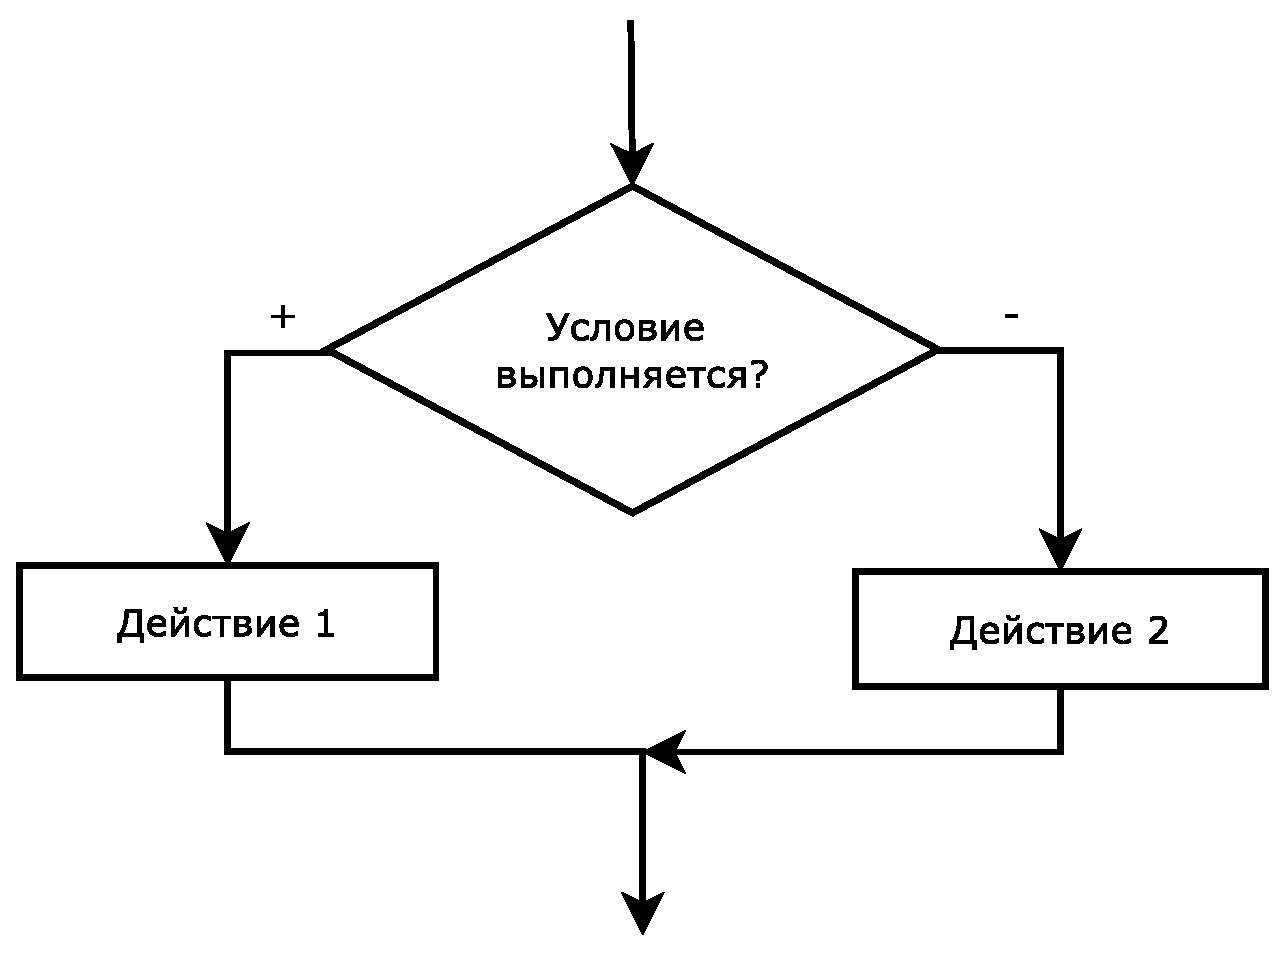
\includegraphics[width=0.5\textwidth]{img/ris_3_8}
%\caption{Алгоритм условного оператора \Sys{if … else}}
%\label{ch03:refDrawing7}
%\end{center}
%\end{figure}

Например, чтобы сравнить значения переменных \Sys{a} и \Sys{b} нужно написать следующий
программный код:
\begin{lstlisting}
cin>>a; cin>>b;
if (a==b) cout<<"a `\Sys{равно}` b";
else cout<<"a `\Sys{не равно}` b";
\end{lstlisting}

\Emph{Внимание!} Не путайте знак проверки равенства \Sys{==} и оператор присваивания
\Sys{=}. Например, в записи \Sys{if (a=0) b=1;} синтаксической ошибки нет. Операция
присваивания \Sys{a=0} формирует результат и его значение проверяется в качестве условия. В данном примере
присваивание \Sys{b=1} не будет выполнено никогда, так как переменная \Sys{a} всегда будет
принимать значение равное нулю, то есть ложь. Верная запись: 
\Sys{if (a==0) b=1;}.

%%%% рис 8 и 9 бок о бок
\begin{figure}[H]
\begin{floatrow}
\floatbox{figure}[.45\textwidth][\FBheight][t]
{\caption{Алгоритм условного оператора \Sys{if … else}}
\label{ch03:refDrawing7}}
{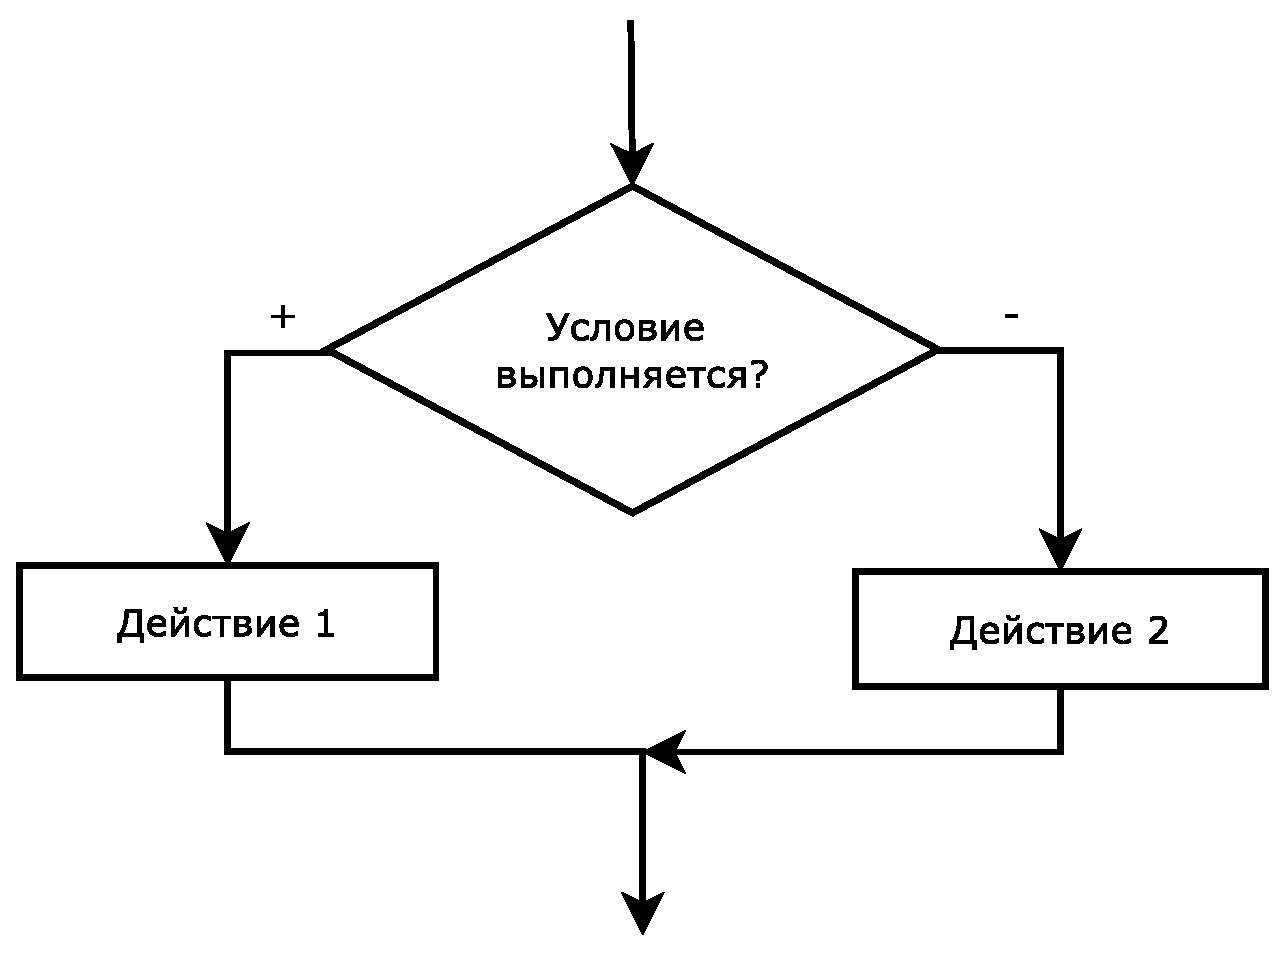
\includegraphics[width=0.45\textwidth,keepaspectratio]{img/ris_3_8}}\hspace*{0.05\textwidth}
%
\floatbox{figure}[.45\textwidth][\FBheight][b]
{\caption{Алгоритм условного оператора \Sys{if}}
\label{ch03:refDrawing8}}
{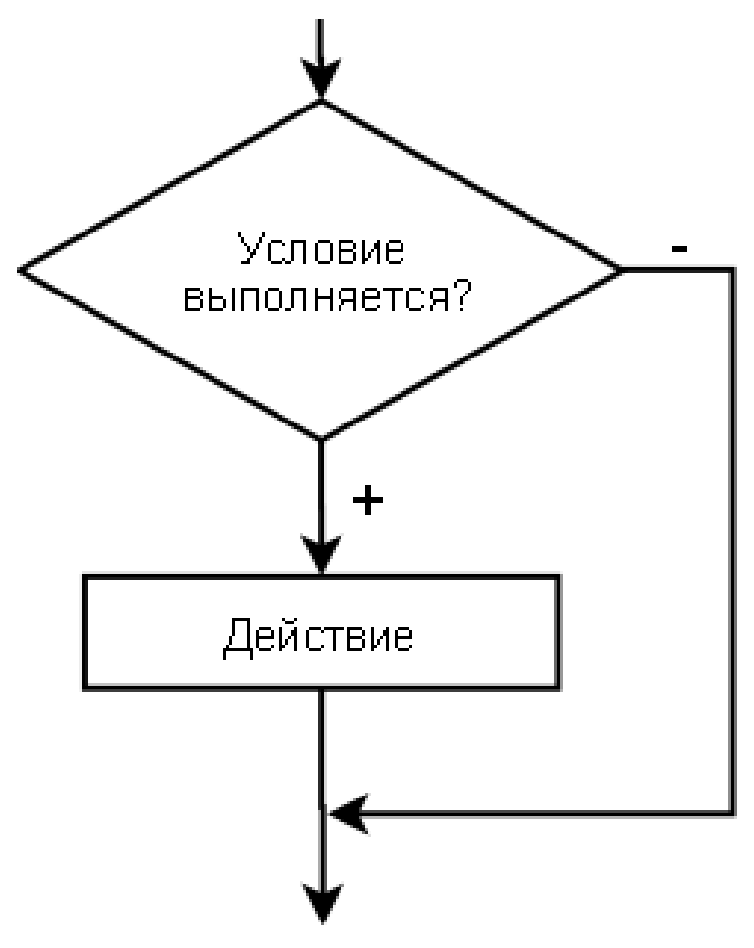
\includegraphics[width=0.35\textwidth]{img/ris_3_9}}
\end{floatrow}
\end{figure}

\Emph{Внимание!} Если в задаче требуется, чтобы в зависимости от значения условия выполнялся не один оператор, а
несколько, их необходимо заключать в фигурные скобки, как составной оператор. В этом случае компилятор воспримет группу
операторов как один:
\begin{lstlisting}
if (`\Sys{условие}`) 
{
  `\Sys{оператор\_1;}`
  `\Sys{оператор\_2;}`
    `…`
}
else 
{
  `\Sys{оператор\_3;}`
  `\Sys{оператор\_4;}`
    `…`
}
\end{lstlisting}

Альтернативная ветвь \Sys{else} в условном операторе может отсутствовать, если в ней нет необходимости: 
\begin{lstlisting}
if (`\Sys{условие}`) `\Sys{оператор;}`
\end{lstlisting}
или
\begin{lstlisting}
if (`\Sys{условие}`)
{
  `\Sys{оператор\_1;}`
  `\Sys{оператор\_2;}`
  `\Sys{…}`
}
\end{lstlisting}

В таком <<усечённом>> виде условный оператор работает так: \Sys{оператор} (группа операторов) либо
выполняется, либо пропускается, в зависимости от значения выражения, представляющего условие. Алгоритм этого условного
процесса представлен на рис.~\ref{ch03:refDrawing8}.


%\begin{figure}[htb]
%\begin{center}
%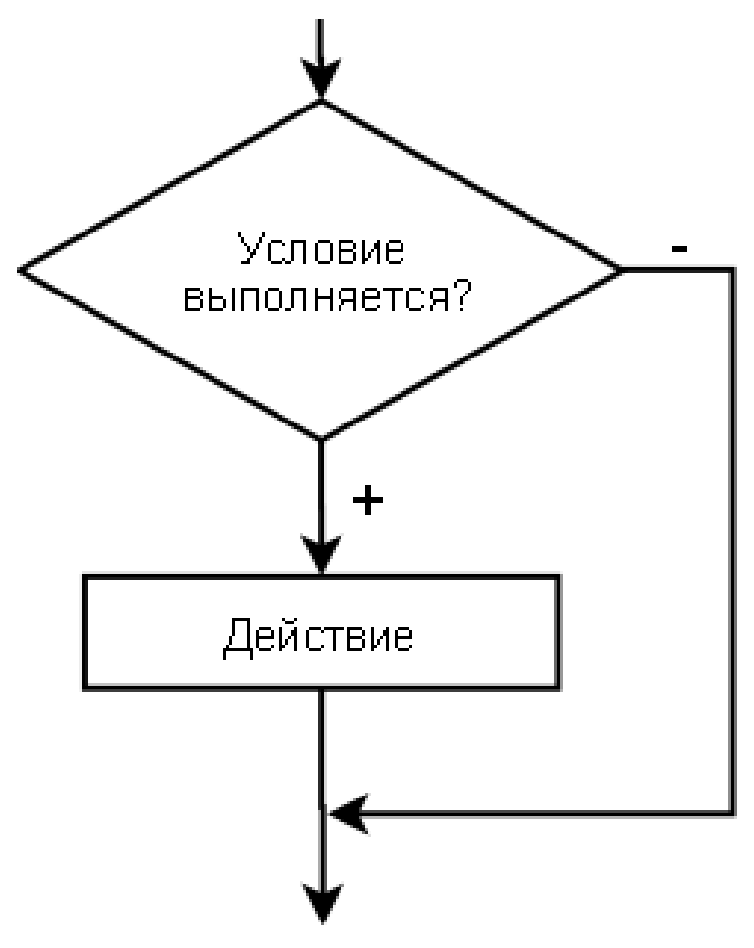
\includegraphics[width=0.5\textwidth]{img/ris_3_9}
%\caption{Алгоритм условного оператора \Sys{if}}
%\label{ch03:refDrawing8}
%\end{center}
%\end{figure}

Пример применения условного оператора без альтернативной ветви \Sys{else} может быть таким:

\begin{lstlisting}
cin>>a; cin>>b;
c=0;
//`Значение переменной \Sys{c} изменяется только при условии, что \Sys{a} не равно \Sys{b}`
if (a!=b) c=a+b;
cout<<"c="<<c;
\end{lstlisting}

Условные операторы могут быть вложены друг в друга. При вложениях условных операторов всегда действует правило:
альтернатива \Sys{else} считается принадлежащей ближайшему \Sys{if}. Например, в записи
\begin{lstlisting}
if `(условие\_1)` if `(условие\_2) оператор\_А`; else `оператор\_Б;`
\end{lstlisting}
\Sys{оператор\_Б} относится к \Sys{условию\_2}, а в конструкции
\begin{lstlisting}
if `(условие\_1)` {if `(условие\_2) оператор\_А`;} 
else `оператор\_Б;`
\end{lstlisting}
он принадлежит оператору \Sys{if} с \Sys{условием\_1}. 

Рассмотрим несколько задач с применением условных процессов.

\prg{Дано вещественное число $x$. Для
функции, график которой приведён на рис.~\ref{ch03:refDrawing9}, вычислить
$y=f(x)$.}{ch03:prg0}

\begin{figure}[htb]
\begin{center}
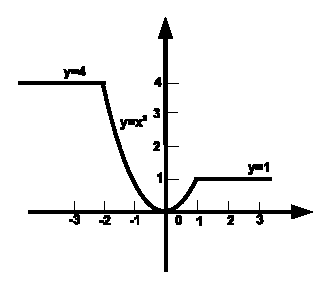
\includegraphics[width=0.5\textwidth]{img/ris_3_10}
\caption{Графическое представление задачи \ref{ch03:prg0}}
\label{ch03:refDrawing9}
\end{center}
\end{figure}

Аналитически функцию, представленную на рис.~\ref{ch03:refDrawing9}, можно записать так:

\begin{equation*}
y(x)=\left\{\begin{matrix}
4, & x\leqslant -2\\
1, & x\geqslant 1\\
x^2, & -2<x<1
\end{matrix}\right.
\end{equation*}

Составим словесный алгоритм решения этой задачи:

\begin{enumerate}
\item Начало алгоритма.
\item Ввод числа $x$ (аргумент функции).
\item Если значение $x$ меньше либо равно -2, то переход к п.~4, иначе переход к~п.~5.
\item Вычисление значения функции: $y=4$, переход к~п.~8.
\item Если значение $x$ больше либо равно 1, то переход к п.~6, иначе переход к~п.~7.
\item Вычисление значения функции: $y=1$, переход к~п.~8.
\item Вычисление значения функции: $y=x^2$.
\item Вывод значений аргумента $x$ и функции $y$.
\item Конец алгоритма.
\end{enumerate}

Блок-схема, соответствующая описанному алгоритму, представлена на рис.~\ref{ch03:refDrawing10}.

\begin{figure}[htb]
\begin{center}
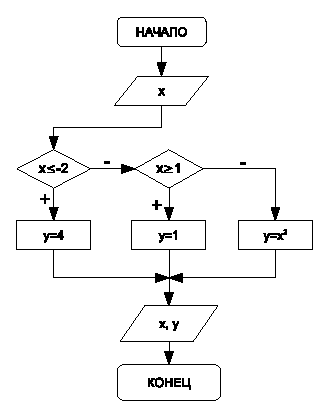
\includegraphics[width=0.5\textwidth]{img/ris_3_11}
\caption{Блок-схема алгоритма решения задачи~\ref{ch03:prg0}}
\label{ch03:refDrawing10}
\end{center}
\end{figure}

Текст программы на языке \Sys{C++} будет иметь вид:
\begin{lstlisting}
#include <iostream>
using namespace std;
int main()
{
  float X,Y;
  cout<<"X="; cin>>X;
  if (X<=-2) Y=4;
  else if (X>=1) Y=1;
  else Y=X*X;
  cout <<"Y=" <<Y<< endl;
  return 0;
}
\end{lstlisting}

\prg{Даны вещественные числа $x$ и $y$. Определить, принадлежит ли точка с координатами ($x$; $y$)
заштрихованной области (рис.~\ref{ch03:refDrawing11}).}{ch03:prg1}

%\begin{figure}[htb]
%\begin{center}
%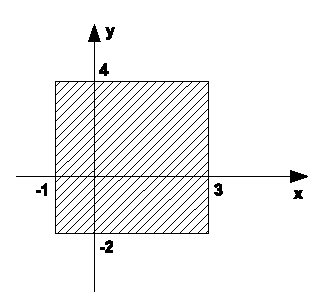
\includegraphics[width=0.3\textwidth]{img/ris_3_12}
%\caption{Графическое представление задачи~\ref{ch03:prg1}}
%\label{ch03:refDrawing11}
%\end{center}
%\end{figure}

%%%% рис 12 и 13 бок о бок
\begin{figure}[H]
\begin{floatrow}
\floatbox{figure}[.35\textwidth][\FBheight][t]
{\caption{Графическое представление задачи~\ref{ch03:prg1}}
\label{ch03:refDrawing11}}
{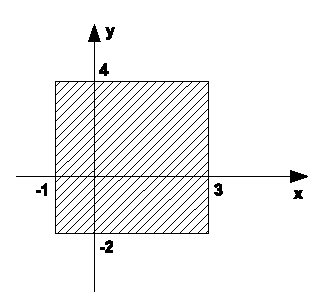
\includegraphics[width=0.3\textwidth,keepaspectratio]{img/ris_3_12}}\hspace*{0.05\textwidth}
%
\floatbox{figure}[.45\textwidth][\FBheight][b]
{\caption{Алгоритм решения задачи~\ref{ch03:prg1}}
\label{ch03:refDrawing12}}
{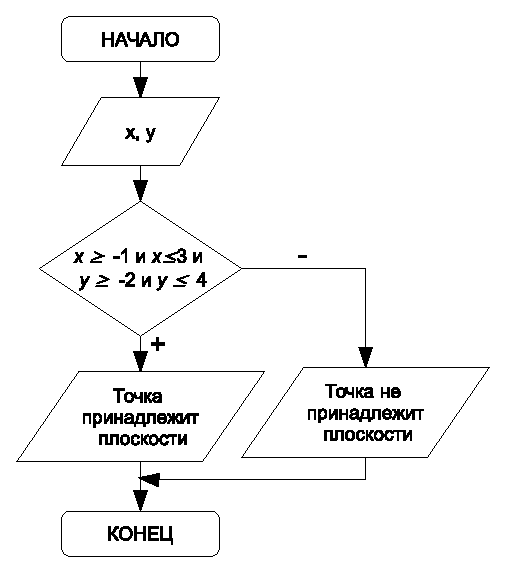
\includegraphics[width=0.4\textwidth]{img/ris_3_13}}
\end{floatrow}
\end{figure}


Как показано на рис.~\ref{ch03:refDrawing11}, область ограничена линиями $x=-1$, $x=3$,
$y=-2$ и $y=4$. Значит точка с координатами ($x$;
$y$) будет принадлежать этой области, если будут выполняться следующие условия: 
$x\geqslant -1$, $x\leqslant 3$, $y\geqslant -2$ и $y\leqslant 4$. Иначе точка лежит за пределами области.

Блок-схема, описывающая алгоритм решения данной задачи, представлена на рис.~\ref{ch03:refDrawing12}.

%\begin{figure}[htb]
%\begin{center}
%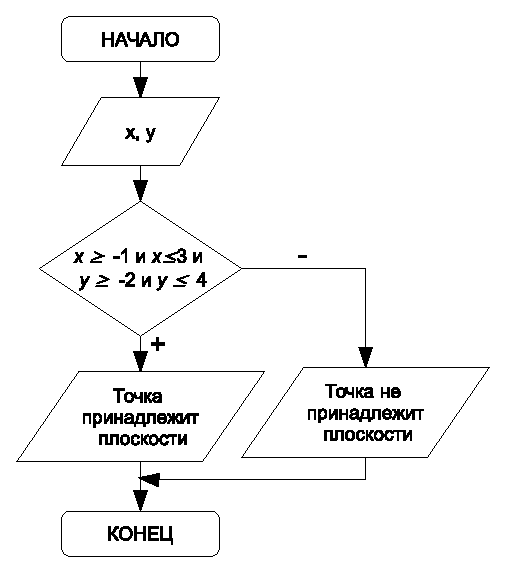
\includegraphics[width=0.4\textwidth]{img/ris_3_13}
%\caption{Алгоритм решения задачи~\ref{ch03:prg1}}
%\label{ch03:refDrawing12}
%\end{center}
%\end{figure}

Текст программы к задаче~\ref{ch03:prg1}:
\begin{lstlisting}
#include <iostream>
using namespace std;
int main()
{float X,Y;
cout<<"X="; cin>>X;
cout<<"Y="; cin>>Y;
if (X>=-1 && X<=3 && Y>=-2 && Y<=4)
  cout <<"`\Sys{Точка принадлежит области}`"<< endl;
else 
  cout<<"`\Sys{Точка не принадлежит области}`"<<endl;
return 0;
}
\end{lstlisting}

\prg{Даны вещественные числа $x$ и $y$. Определить, принадлежит ли точка с координатами ($x$; $y$)
заштрихованной области (рис.~\ref{ch03:refDrawing13}).}{ch03:prg3}

\begin{figure}[htb]
\begin{center}
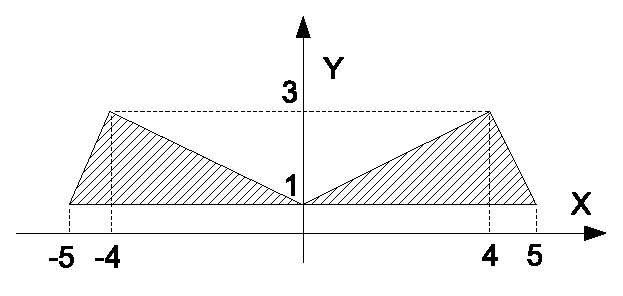
\includegraphics[width=0.5\textwidth]{img/ris_3_14}
\caption{Графическое представление задачи~\ref{ch03:prg3}}
\label{ch03:refDrawing13}
\end{center}
\end{figure}

Составим уравнения линий, ограничивающих заданные области. В общем виде уравнение прямой, проходящей через точки с
координатами  $(x_1,y_1)$ и  $(x_2,y_2)$,  имеет вид:

 $$\frac{x-x_1}{x_2-x_1}=\frac{y-y_1}{y_2-y_1}$$.

Треугольник в первой координатной области ограничен линиями, проходящими через точки:

\begin{enumerate}
\item $(0, 1) - (4, 3)$;
\item $(4, 3) - (5, 1)$;
\item $(5, 1) - (0, 1)$.
\end{enumerate}
Следовательно, уравнение первой линии:

 $$\frac{x-0}{4-0}=\frac{y-1}{3-1}\Rightarrow \frac{x}{4}=\frac{y-1}{2}\Rightarrow y=1+\frac{1}{2}\cdot x,$$
уравнение второй линии:
$$
\frac{x-4}{5-4}=\frac{y-3}{1-3}\Rightarrow x-4=\frac{y-3}{-2}\Rightarrow -2\cdot x+8=y-3\Rightarrow y=-2\cdot x+11
$$
и уравнение третьей линии:  $y=1$.

Линии, которые формируют треугольник во второй координатной области, проходят через точки:

\begin{enumerate}
\item $(0, 1) - (-4, 3)$;
\item $(-4, 3) - (-5, 1)$;
\item $(-5, 1) - (0, 1)$;
\end{enumerate}
Следовательно, уравнение первой линии:
 $$\frac{x-0}{-4-0}=\frac{y-1}{3-1}\Rightarrow \frac{x}{-4}=\frac{y-1}{2}\Rightarrow y=1-\frac{1}{2}\cdot x,$$
уравнение второй линии:
$$
\frac{x+4}{-5+4}=\frac{y-3}{1-3}\Rightarrow \frac{x+4}{-1}=\frac{y-3}{-2}\Rightarrow -2\cdot x-8=-y+3\Rightarrow
y=2\cdot x+11
$$
и уравнение третьей линии:  $y=1$.

Таким образом, условие попадания точки в заштрихованную часть плоскости имеет вид:

\begin{equation*}
\left\{
\begin{array}{c}
y\leqslant 1+\frac{1}{2}\cdot x\\
y\leqslant -2\cdot x+11\\
y\geqslant 1
\end{array}%
\right.
\ \ \text{или}\ \  
\left\{
\begin{array}{c}
y\leqslant 1-\frac{1}{2}\cdot x\\
y\leqslant 2\cdot x+11\\
y\geqslant 1
\end{array}
\right. 
\end{equation*}

Далее приведён текст программы для решения задачи \ref{ch03:prg3}.

\begin{lstlisting}
#include <iostream>
using namespace std;
int main()
{
	float X,Y;
	cout<<"X=";
	cin>>X;
	cout<<"Y=";
	cin>>Y;
	if ((Y<=1+(float)1/2*X && Y<=-2*X+11 && Y>=1) || (Y<=1-(float)1/2*X && Y<=2*X+11 && Y>=1))
		cout << `\Sys{"Точка принадлежит области"}` << endl;
	else
		cout << `\Sys{"Точка не принадлежит области"}` << endl;
	return 0;
}
\end{lstlisting}

\prg{Написать программу решения квадратного уравнения\\
$ax^2+bx+c=0$.}{ch03:prg4} 

Исходные данные: вещественные числа $a$, $b$ и $c$ --- коэффициенты
квадратного уравнения.

Результаты работы программы: вещественные числа $x1$ и $x2$ --- корни квадратного
уравнения либо сообщение о том, что корней нет.

Вспомогательные переменные: вещественная переменная $d$, в которой будет храниться дискриминант
квадратного уравнения.

Составим словесный алгоритм решения этой задачи.
\begin{enumerate}
\item Начало алгоритма.
\item Ввод числовых значений переменных $a$, $b$ и $c$.
\item Вычисление значения дискриминанта $d$ по формуле  $d=b^2-4ac$.
\item Если $d<0$, то переход к п.5, иначе переход к п.6.
\item Вывод сообщения \Sys{"Действительных корней нет"} и переход к п.8.
\item Вычисление корней  $x1=\frac{-b+\sqrt{d}}{2a}$  и  $x2=\frac{-b-\sqrt{d}}{2a}$.
\item Вывод значений $x1$ и $x2$ на экран.
\item Конец алгоритма.
\end{enumerate}
Блок-схема, соответствующая этому описанию, представлена на рис.~\ref{ch03:refDrawing14}.

\begin{figure}[htb]
\begin{center}
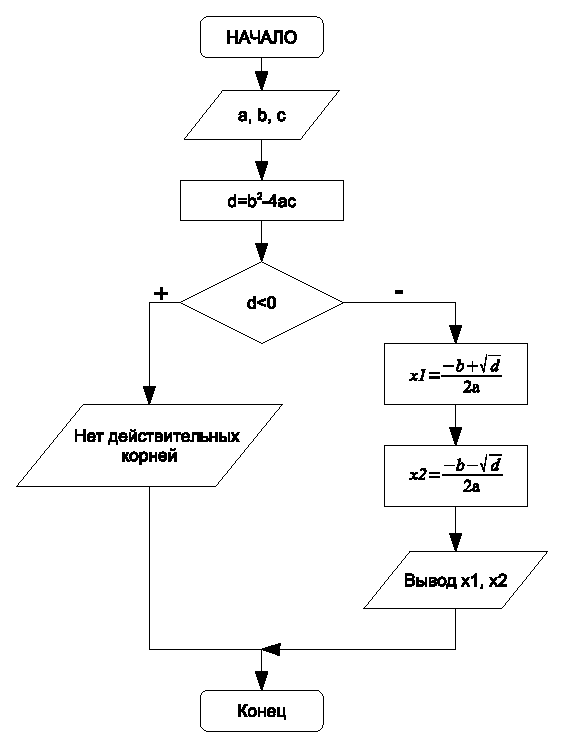
\includegraphics[width=0.7\textwidth]{img/ris_3_15}
\caption{Алгоритм решения квадратного уравнения}
\label{ch03:refDrawing14}
\end{center}
\end{figure}

Текст программы, которая реализует решение квадратного уравнения: 
\begin{lstlisting}
#include <iostream>
#include <math.h>
using namespace std;
int main()
{
float a,b,c,d,x1,x2;
//`Ввод значений коэффициентов квадратного уравнения.`
cout<<"a=";cin>>a;
cout<<"b=";cin>>b;
cout<<"c=";cin>>c;
d=b*b-4*a*c;	//`\Sys{Вычисление дискриминанта.}`
if (d<0)        
//`Если дискриминант отрицательный, то вывод сообщения, о том что действительных корней нет,`
  cout<<"`\Sys{Нет действительных корней}`";
else
{
//`иначе вычисление действительных корней`
  x1=(-b+sqrt(d))/2/a;
  x2=(-b-sqrt(d))/(2*a);
//`и вывод их значений.`
  cout<<"X1="<<x1<<"\t X2="<<x2<<"\n";
}
return 0;
}
\end{lstlisting}

\prg{Составить программу нахождения действительных и
комплексных корней квадратного уравнения
$ax^2+bx+c=0$.}{ch03:prg5} 

Исходные данные: вещественные числа $a$, $b$ и $c$ --- коэффициенты
квадратного уравнения.

Результаты работы программы: вещественные числа $x1$ и $x2$ --- действительные корни
квадратного уравнения либо $x1$ и $x2$ --- действительная и мнимая части комплексных
корней квадратного уравнения.

Вспомогательные переменные: вещественная переменная $d$, в которой будет храниться дискриминант
квадратного уравнения.

Можно выделить следующие этапы решения задачи:
\begin{enumerate}
\item Ввод коэффициентов квадратного уравнения $a$, $b$ и $c$.
\item Вычисление дискриминанта $d$ по формуле  $d=b^2-4ac$.
\item Проверка знака дискриминанта. Если $d\geqslant 0$, то вычисление действительных корней:
 $x1=\frac{-b+\sqrt{d}}{2a}$  и  $x2=\frac{-b-\sqrt{d}}{2a}$ 
и вывод их на экран. При отрицательном дискриминанте выводится сообщение о том, что действительных корней нет, и
вычисляются комплексные корни\footnote{Комплексные числа записываются в виде
$a+ib$, где $a$ --- действительная часть комплексного числа,
$b$ --- мнимая часть комплексного числа, $i$ --- мнимая единица  $\sqrt{-1}$. Подробно о комплексных числах можно прочитать в главе~\ref{ch09}.}
 $x1=\frac{-b}{2a}+i\frac{\sqrt{\left|{d}\right|}}{2a}$, 
$x2=\frac{-b}{2a}-i\frac{\sqrt{\left|{d}\right|}}{2a}$.
\end{enumerate}

У обоих комплексных корней действительные части одинаковые, а мнимые отличаются знаком. Поэтому можно в переменной
$x1$ хранить действительную часть числа  $\frac{-b}{2a}$, в переменной $x2$ --- модуль мнимой части 
$\frac{\sqrt{\left|{d}\right|}}{2a}$, а в качестве корней вывести 
$x1 + i\cdot x2$  и  $x1 - i\cdot x2$. 

На рис.~\ref{ch03:refDrawing15} изображена блок-схема решения задачи. Блок~1 предназначен для ввода коэффициентов квадратного
уравнения. В блоке~2 осуществляется вычисление дискриминанта. Блок~3 осуществляет проверку знака дискриминанта, если
дискриминант отрицателен, то корни комплексные, их расчёт происходит в блоке~4 (действительная часть корня записывается
в переменную $x1$, модуль мнимой --- в переменную $x2$), а вывод --- в блоке~5 (первый
корень $x1 + i\cdot x2$, второй --- $x1 - i\cdot x2$). Если дискриминант положителен, то
вычисляются действительные корни уравнения (блок~6) и выводятся на экран (блок~7).

\begin{figure}[htb]
\begin{center}
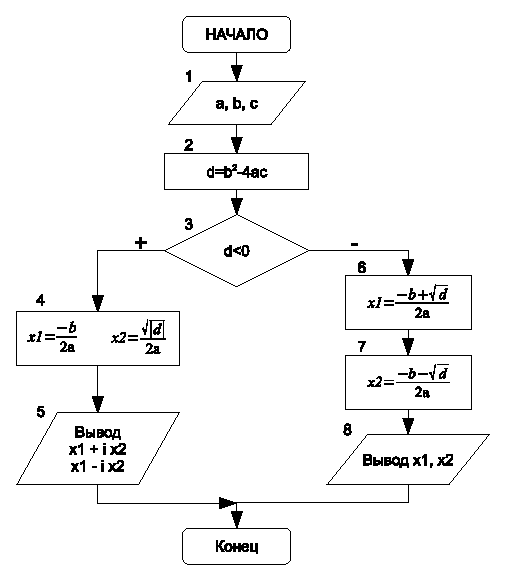
\includegraphics[width=0.7\textwidth]{img/ris_3_16}
\caption{Алгоритм решения задачи \ref{ch03:prg5}}
\label{ch03:refDrawing15}
\end{center}
\end{figure}

Текст программы, реализующей поставленную задачу:
\begin{lstlisting}
#include <iostream>
#include <math.h>
using namespace std;
int main()
{
float a,b,c,d,x1,x2;
cout<<"a=";cin>>a;
cout<<"b=";cin>>b;
cout<<"c=";cin>>c;
d=b*b-4*a*c;
if (d<0)
{//`\Sys{Если дискриминант отрицательный, то вывод соответствующего сообщения.}`
  cout<<"`\Sys{Нет вещественных корней }`\n";
  x1=-b/(2*a);  //`\Sys{Вычисление действительной части комплексных корней.}`
  x2=sqrt(fabs(d))/(2*a); //`\Sys{Вычисление модуля мнимой части комплексных корней}`
  //`\Sys{Сообщение о комплексных корнях уравнения вида} $ax^2+bx+c=0$.`
  cout<<"`\Sys{Комплексные корни уравнения}` \n";
  cout<<a<<"x^2+"<<b<<"x+"<<c<<"=0 \n";
  //`\Sys{Вывод значений комплексных корней в виде $x1\pm ix2$}`
  if (x2>=0)
  {
    cout<<x1<<"+"<<x2<<"i\t";
    cout<<x1<<"-"<<x2<<"i\n";
  }
  else
  {
    cout<<x1<<"-"<<fabs(x2)<<"i\t";
    cout<<x1<<"+"<<fabs(x2)<<"i\n";
  }
}
else
{
//`\Sys{Если дискриминант положительный, вычисление действительных корней и вывод их на экран.}`
  x1=(-b+sqrt(d))/2/a;
  x2=(-b-sqrt(d))/(2*a);
  cout<<"`\Sys{Вещественные корни уравнения}` \n";
  cout<<a<<"x^2+"<<b<<"x+"<<c<<"=0 \n";
  cout<<"X1="<<x1<<"\t X2="<<x2<<"\n";
}
return 0;
}
\end{lstlisting}

Результаты работы программы к задаче~\ref{ch03:prg5} показаны ниже.%рис. \ref{ch03:refDrawing16} и \ref{ch03:refDrawing17}.
\begin{verbatim}
a=-5
b=-3
c=-4
Нет вещественных корней 
Комплексные корни уравнения 
-5x^2+-3x+-4=0 
-0.3-0.842615i	-0.3+0.842615i
==============================
a=2
b=-3
c=1
Вещественные корни уравнения 
2x^2+-3x+1=0 
X1=1	 X2=0.5
\end{verbatim}


\prg{Составить программу для решения кубического уравнения\\
$ax^3+bx^2+cx+d=0$.}{ch03:prg6}

Кубическое уравнение имеет вид
\begin{equation}\label{ch03:eq1}
ax^3+bx^2+cx+d=0
\end{equation}

После деления на $a$ уравнение~\ref{ch03:eq1} принимает канонический вид:
\begin{equation}\label{ch03:eq2}
x^{3}+rx^2+sx+t=0,
\end{equation}
где $r=\frac{b}{a}$, $s=\frac{c}{a}$, $t=\frac{d}{a}$. 

В уравнении~\ref{ch03:eq2} сделаем замену  $x=y-\frac{r}{3}$  и получим приведённое уравнение:
\begin{equation}\label{ch03:eq3}
y^3+py+q=0,
\end{equation}
где $p=\frac{3s-r^2}{3}$,  $q=\frac{2r^3}{27}-\frac{rs}{3}+t$.

Число действительных корней приведённого уравнения (\ref{ch03:eq3}) зависит от знака дискриминанта (табл.
\ref{ch03:refTable0})
 $D=(\frac{p}{3})^3+(\frac{q}{2})^2$.

{\tabcolsep=0.3em\noindent\small
\begin{longtable}{|p{0.2\textwidth}|p{0.33\textwidth}|p{0.35\textwidth}|}
\caption{Количество корней кубического уравнения} \label{ch03:refTable0}\\
\hline
\Emph{Дискрими\-нант}&\Emph{Количество действительных корней}&\Emph{Количество комплексных корней}\\
\hline \hline
\endfirsthead
\multicolumn{3}{c}%
{{\tablename\ \thetable{} --- продолжение}} \\
\hline
\Emph{Дискрими\-нант}&\Emph{Количество действительных корней}&\Emph{Количество комплексных корней}\\
\hline \hline
\endhead
\centering $D\geqslant 0$ & \centering 1 & \centering 2\tabularnewline\hline
\centering $D<0$ & \centering 3 & \centering\ $-$\tabularnewline\hline
\end{longtable}
}

Корни приведённого уравнения могут быть рассчитаны по формулам Кардано:

\begin{equation}\label{ch03:eq4}
\begin{array}{l}
y_1=u+v\\
y_2=\frac{-{u+v}}{2}+\frac{u-v}{2}i\sqrt{3}\\
y_3=\frac{-{u+v}}{2}-\frac{u-v}{2}i\sqrt{3},
\end{array}
\end{equation}
где $u=\sqrt[{3}]{\frac{-q}{2}+\sqrt{D}}$,\ \  $v=\sqrt[{3}]{\frac{-q}{2}-\sqrt{D}}$.

При отрицательном дискриминанте уравнение (\ref{ch03:eq1}) имеет три действительных корня, но они будут вычисляться
через вспомогательные комплексные величины. Чтобы избавиться от этого, можно воспользоваться формулами:
\begin{equation}\label{ch03:eq5}
\begin{array}{l}
y_1=2\sqrt[{3}]{\rho}\cos(\frac{\phi}{3}),\\
y_2=2\sqrt[{3}]{\rho}\cos(\frac{\phi}{3}+\frac{2\pi}{3}),\\
y_3=2\sqrt[{3}]{\rho}\cos(\frac{\phi}{3}+\frac{4\pi}{3}),
\end{array}
\end{equation}
где $\rho =\sqrt{\frac{-{p^{3}}}{27}},\ \ \cos(\phi )=\frac{-{q}}{2\rho}$.

Таким образом, при положительном дискриминанте кубического уравнения (\ref{ch03:eq3}) расчёт корней будем вести по
формулам (\ref{ch03:eq4}), а при отрицательном --- по формулам (\ref{ch03:eq5}). После расчёта корней приведённого
уравнения (\ref{ch03:eq3}) по формулам (\ref{ch03:eq4}) или (\ref{ch03:eq5}), необходимо по формулам 

\begin{equation*}
x_{k}=y_{k}-\frac{r}{3},\ k=1,2,3..,
\end{equation*}
перейти к корням заданного кубического уравнения (\ref{ch03:eq1}).

Блок-схема решения кубического уравнения представлена на рис.~\ref{ch03:refDrawing19}.

\begin{figure}[ht]
\begin{center}
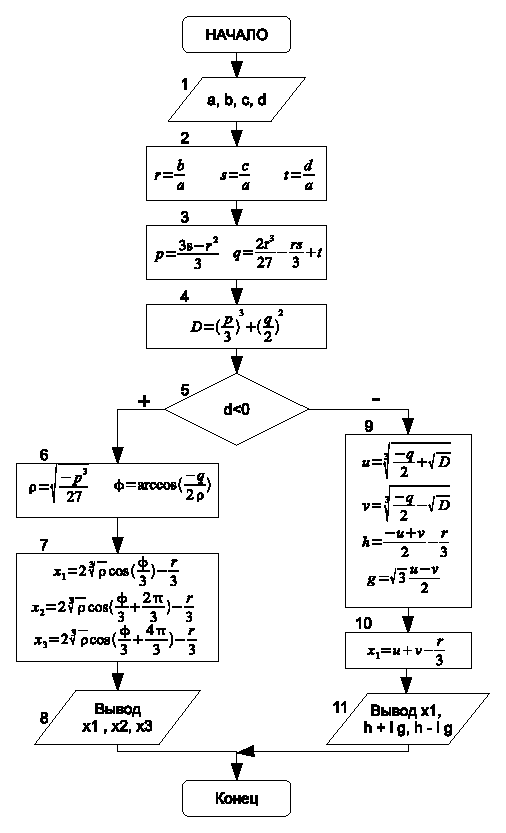
\includegraphics[width=0.6\textwidth]{img/ris_3_19}
\caption{Алгоритм решения кубического уравнения}
\label{ch03:refDrawing18}
\end{center}
\end{figure}

Описание блок-схемы. В блоке 1 вводятся коэффициенты кубического уравнения, в блоках 2--3 рассчитываются коэффициенты
канонического и приведённого уравнений. Блок 4 предназначен для вычисления дискриминанта. В блоке 5 проверяется знак
дискриминанта кубического уравнения. Если он отрицателен, то корни вычисляются по формулам~\ref{ch03:eq5} (блоки 6--7). При
положительном значении дискриминанта расчёт идёт по формулам~\ref{ch03:eq4} (блок 9, 10). Блоки 8 и 11 предназначены для вывода результатов на экран.

Текст программы с комментариями приведён ниже\footnote{При расчёте величин \Sys{u} и \Sys{v} в
программе предусмотрена проверка значения подкоренного выражения. 

Если  $\frac{-q}{2}\mp\sqrt{D}>0$,\ \ то\ \ $u=\sqrt[{3}]{\frac{-q}{2}+\sqrt{D}}$, 
а \ \ $v=\sqrt[{3}]{\frac{-q}{2}-\sqrt{D}}$.

Если  $\frac{-q}{2}\mp\sqrt{D}<0$,\ \ то\ \ $u=\sqrt[{3}]{|\frac{-q}{2}+\sqrt{D}|}$,
\ \  а\ \ $v=\sqrt[{3}]{|\frac{-q}{2}-\sqrt{D}|}$.

Соответственно, при нулевом значении подкоренного выражения \Sys{u} и \Sys{v} обращаются
в ноль}.

\begin{lstlisting}
#include <iostream>
#include <math.h>
using namespace std;
#define pi 3.14159  //`\Sys{Определение константы}`
int main()
{
float a,b,c,d,D,r,s,t,p,q,ro,fi,x1,x2,x3,u,v,h,g;
//`\Sys{Ввод коэффициентов кубического уравнения.}`
cout<<"a="; cin>>a;
cout<<"b="; cin>>b;
cout<<"c="; cin>>c;
cout<<"d="; cin>>d;
//`\Sys{Расчёт коэффициентов канонического уравнения по формуле~\ref{ch03:eq2}}`
r=b/a; s=c/a; t=d/a;
//`\Sys{Вычисление коэффициентов приведённого уравнения по формуле~\ref{ch03:eq3}}`
p=(3*s-r*r)/3; q=2*r*r*r/27-r*s/3+t;
//`\Sys{Вычисление дискриминанта кубического уравнения}`
D=(p/3)*(p/3)*(p/3)+(q/2)*(q/2);
if (D<0)
{
  //`\Sys{Формулы ~\ref{ch03:eq5}}`
  ro=sqrt((float)(-p*p*p/27));
  fi=-q/(2*ro);
  fi=pi/2-atan(fi/sqrt(1-fi*fi));
  x1=2*pow(ro,(float)1/3)*cos(fi/3)-r/3;
  x2=2*pow(ro,(float)1/3)*cos(fi/3+2*pi/3)-r/3;
  x3=2*pow(ro,(float)1/3)*cos(fi/3+4*pi/3)-r/3;
  cout<<"\n x1="<<x1<<"\t x2="<<x2;
  cout<<"\t x3="<<x3<<"\n";
}
else
{
  //`\Sys{Формулы ~\ref{ch03:eq4}}`
  if (-q/2+sqrt(D)>0) u=pow((-q/2+sqrt(D)),(float)1/3);
  else 
  if (-q/2+sqrt(D)<0) u=-pow(fabs(-q/2+sqrt(D)),(float)1/3);
  else u=0;
  if (-q/2-sqrt(D)>0) v=pow((-q/2-sqrt(D)),(float)1/3);
  else
  if (-q/2-sqrt(D)<0) v=-pow(fabs(-q/2-sqrt(D)),(float)1/3);
  else v=0;
    x1=u+v-r/3; //`\Sys{Вычисление действительного корня кубического уравнения.}`
    h=-(u+v)/2-r/3; //`\Sys{Вычисление действительной}` 
    g=(u-v)/2*sqrt((float)3); //`\Sys{и мнимой части комплексных корней}`
    cout<<"\n x1="<<x1;
    if (x2>=0)
      {
        cout<<x1<<"+"<<x2<<"i\t";
        cout<<x1<<"-"<<x2<<"i\n";
      }
    else
      {
        cout<<x1<<"-"<<fabs(x2)<<"i\t";
        cout<<x1<<"+"<<fabs(x2)<<"i\n";
      }
    }
if (g>=0)
{
cout<<"\t x2="<<h<<"+"<<g<<"i";
cout<<"\t x3="<<h<<"-"<<g<<"i \n";
}
else
{
cout<<"\t x2="<<h<<"-"<<fabs(g)<<"i";
cout<<"\t x2="<<h<<"+"<<fabs(g)<<"i";
}
}
return 0;
}
\end{lstlisting}


\prg{Заданы коэффициенты $a$, $b$ и $c$ биквадратного уравнения
$ax^4+bx^2+c=0$. Найти все его действительные корни.}{ch03:prg7}

\emph{Входные данные}: $a$, $b$, $c$.

\emph{Выходные данные}: $x1$, $x2$, $x3$, $x4$.

Для решения биквадратного уравнения необходимо заменой $y=x^2$
привести его к квадратному уравнению
$ay^2+by+c=0$ и решить это уравнение.

Опишем алгоритм решения этой задачи (рис.~\ref{ch03:refDrawing19}):
\begin{enumerate}
\item Ввод коэффициентов биквадратного уравнения $a$, $b$ и $c$ (блок~1).
\item Вычисление дискриминанта уравнения $d$ (блок~2).
\item Если $d<0$ (блок~3), вывод сообщения, что корней нет (блок~4), а иначе определяются
корни соответствующего квадратного уравнения $y1$ и $y2$ (блок~5).
\item Если $y1<0$ и $y2<0$ (блок~6) , то вывод сообщения, что корней нет (блок~7).
\item Если $y1\geq 0$ и $y2\geq 0$ (блок~8), то вычисляются четыре корня по формулам  
$\pm\sqrt{y_1}, \pm\sqrt{y_2}$ (блок~9) и выводятся значения корней (блок~10).
\item Если условия 4) и 5) не выполняются, то необходимо проверить знак $y1$. Если
$y1\geq 0$ (блок~11), то вычисляются два корня по формуле  $\pm\sqrt{y_1}$ (блок~12), 
иначе (если  $y2\geq 0$) вычисляются два корня по формуле  $\pm\sqrt{y_2}$ (блок~13). Вывод вычисленных
значений корней (блок 14).
\end{enumerate}

\begin{figure}[ht]
\begin{center}
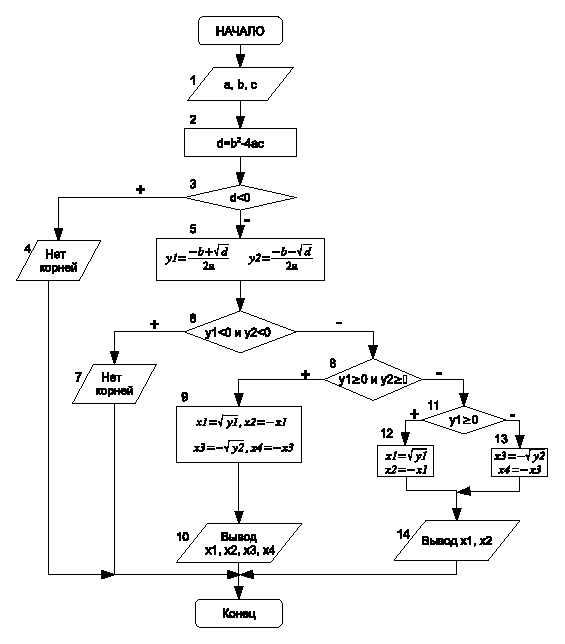
\includegraphics[width=0.7\textwidth]{img/ris_3_20}
\caption{Алгоритм решения биквадратного уравнения}
\label{ch03:refDrawing19}
\end{center}
\end{figure}

Текст программы решения биквадратного уравнения приведён ниже.

\Emph{Внимание!} Если в условном операторе проверяется двойное условие, необходимо применять логические операции
\Sys{{\textbar}{\textbar}}, \Sys{\&\&}, \Sys{!}. Например, условие «если
$y1$ и $y2$ положительны» правильно записать так: \Sys{if (y1{\textgreater}=0 \&\& y2{\textgreater}=0)}.
\begin{lstlisting}
#include <iostream>
#include <math.h>
using namespace std;

int main()
{//`Описание переменных:`
 //a,b,c - `коэффициенты биквадратного уравнения,`
 //d - `дискриминант,`
 //x1,x2,x3,x4 - `корни биквадратного уравнения,`
 //y1,y2 - `корни квадратного уравнения` ay^2+by+c=0,
 float a,b,c,d,x1,x2,x3,x4,y1,y2;
 //`Ввод коэффициентов уравнения.`
 cout<<"a="; cin>>a;
 cout<<"b="; cin>>b;
 cout<<"c="; cin>>c;
 d=b*b-4*a*c;  //`Вычисление дискриминанта.`
 if (d<0)  //`Если дискриминант отрицательный, вывод сообщения «Корней нет».`
  cout<<"`Нет действительных корней` \n";
 else  //`Если дискриминант положительный`,
 {
 //`Вычисление корней соответствующего квадратного уравнения`.
   y1=(-b+sqrt(d))/2/a;
   y2=(-b-sqrt(d))/(2*a);
 //`Если оба корня квадратного уравнения отрицательные`,
  if (y1<0 && y2<0)
 //`вывод сообщения «Корней нет»`
     cout<<" `Нет действительных корней` \n";
 //`Если оба корня квадратного уравнения положительные`,
   else if (y1>=0 && y2>=0)
   {//`Вычисление четырёх корней биквадратного уравнения`
    x1=sqrt(y1);
    x2=-x1;
    x3=sqrt(y2);
    x4=-sqrt(y2);
    //`Вывод корней уравнения на экран`.
    cout<<"\t X1="<<x1<<"\t X2="<<x2;
    cout<<"\t X3="<<x3<<"\t X4="<<x4<<"\n";
   }
    //`Если не выполнились условия`
    //1. y1<0 `и` y2<0
    //2. y1>=0 `и` y2>=0,
    //`то проверяем условие` y1>=0.
    else if (y1>=0) //`Если оно истинно`
    { //`вычисляем два корня биквадратного уравнения.`
      x1=sqrt(y1);
      x2=-x1;
      cout<<"X1="<<x1<<"\t X2="<<x2<<"\n";
    }
    else
    { //`Если условие` y1>=0 `ложно, то вычисляем два корня биквадратного уравнения`
      x1=sqrt(y2);
      x2=-x1;
      cout<<"X1="<<x1<<"\t X2="<<x2<<"\n";
    }
  }
return 0;
}
\end{lstlisting}



Читателю предлагается самостоятельно модифицировать программу таким образом, чтобы она находила все корни (как
действительные, так и комплексные) биквадратного уравнения.

\subsection[Оператор варианта]{Оператор варианта}
Оператор варианта \Sys{switch} необходим в тех случаях, когда в зависимости от значений какой-либо
переменной надо выполнить те или иные операторы:
\begin{lstlisting}
switch `\Sys{(выражение)}`
{
case `\Sys{значение\_1: Операторы\_1;}` break;
case `\Sys{значение\_2: Операторы\_2;}` break;
case `\Sys{значение\_3: Операторы\_3;}` break;
  `\Sys{…}`
case `\Sys{значение\_n: Операторы\_n;}` break;
default: `\Sys{Операторы;}` break;
}
\end{lstlisting}

Оператор работает следующим образом. Вычисляется значение выражения (оно должно быть целочисленным). 
Если выражение принимает
\Sys{значение\_1}, то выполняются \Sys{операторы\_1}. Если выражение принимает
\Sys{значение\_2}, то выполняется \Sys{операторы\_2} и так далее. Если выражение не принимает
ни одно из значений, то выполняются операторы, расположенные после ключевого слова \Sys{default}.

Альтернативная ветвь \Sys{default} может отсутствовать, тогда оператор имеет вид:
\begin{lstlisting}
switch `\Sys{(выражение)}`
{
case `\Sys{значение\_1: Операторы\_1;}` break;
case `\Sys{значение\_2: Операторы\_2;}` break;
case `\Sys{значение\_3: Операторы\_3;}` break;
  `\Sys{…}`
case `\Sys{значение\_n: Операторы\_n;}` break;
}
\end{lstlisting}

Оператор \Sys{break} необходим для того, чтобы осуществить выход из оператора \Sys{switch}.
Если оператор \Sys{break} не указан, то будут выполняться следующие операторы из списка, несмотря на то,
что значение, которым они помечены, не совпадает со значением выражения.

Рассмотрим применение оператора варианта.

\prg{Вывести на печать название дня недели, соответствующее
заданному числу $D$, при условии, что в месяце 31 день и 1-е число --- понедельник.}{ch03:prg8}

Для решения задачи воспользуемся операцией \Sys{\%}, позволяющей вычислить остаток от деления двух чисел,
и условием, что 1-е число --- понедельник. Если в результате остаток от деления (обозначим его $R$)
заданного числа $D$ на семь будет равен единице, то это понедельник, двойке --- вторник, тройке --- среда
и так далее. Следовательно, при построении алгоритма необходимо использовать семь условных операторов, как показано
рис.~\ref{ch03:refDrawing20}. Решение задачи станет значительно проще, если при написании 
программы воспользоваться оператором
варианта \Sys{switch}:
\begin{lstlisting}
#include <iostream>
using namespace std;
int main()
{unsigned int D,R; //`Описаны целые положительные числа.`
  cout<<"D="; cin>>D;  //`Ввод числа от 1 до 31.`
  R=D%7;
  switch (R)
  {
    case 1: cout<<"`Понедельник` \n"; break;
    case 2: cout<<"`Вторник` \n"; break;
    case 3: cout<<"`Среда` \n"; break;
    case 4: cout<<"`Четверг` \n"; break;
    case 5: cout<<"`Пятница` \n"; break;
    case 6: cout<<"`Суббота` \n"; break;
    case 0: cout<<"`Воскресенье` \n"; break;
  }
return 0;
}
\end{lstlisting}
\begin{figure}[htb]
\begin{center}
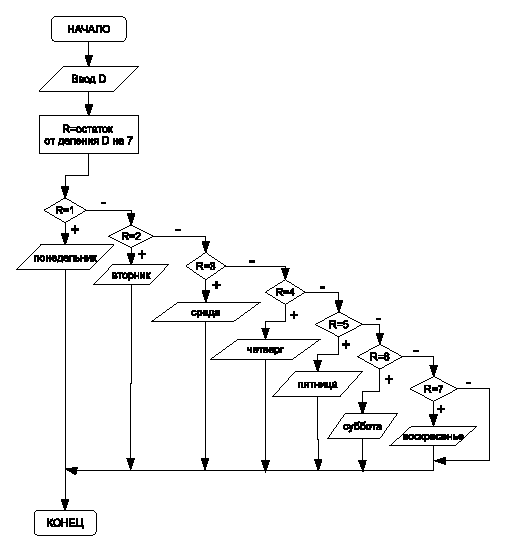
\includegraphics[width=0.7\textwidth]{img/ris_3_21}
\caption{Алгоритм решения задачи \ref{ch03:prg8}}
\label{ch03:refDrawing20}
\end{center}
\end{figure}

В предложенной записи оператора варианта отсутствует ветвь \Sys{default}. Это объясняется тем, что
переменная $R$ может принимать только одно из указанных значений, т.е. 1, 2, 3, 4, 5, 6 или 0. Однако
программа будет работать неправильно, если пользователь введёт значение $D$, превышающее 31. Чтобы
избежать подобной ошибки лучше сделать дополнительную проверку входных данных:
\begin{lstlisting}
#include <iostream>
using namespace std;
int main()
{
unsigned int D,R;
cout<<"\n D="; cin>>D;
if (D<32)  //`Проверка введённого значения.`
{
  R=D%7;
  switch (R)
  {
    case 1: cout<<"`Понедельник` \n"; break;
    case 2: cout<<"`Вторник` \n"; break;
    case 3: cout<<"`Среда` \n"; break;
    case 4: cout<<"`Четверг` \n"; break;
    case 5: cout<<"`Пятница` \n"; break;
    case 6: cout<<"`Суббота` \n"; break;
    case 0: cout<<"`Воскресенье` \n"; break;
  }
}
//`Сообщение об ошибке в случае некорректного ввода.`
else cout<<"`ОШИБКА!` \n";
return 0;
}
\end{lstlisting}

\prg{По заданному номеру месяца $m$ вывести на экран его 
название.}{ch03:prg9}

Для решения данной задачи необходимо проверить выполнение двенадцати условий. 
Если $m$ равно единице, то это январь, если двойке, то февраль, тройке --- март и так далее. 
Понятно, что область возможных значений переменной $m$
находится в диапазоне от 1 до 12 и если пользователь введёт число не входящее в этот интервал, то появится сообщение об
ошибке.
\begin{lstlisting}
#include <iostream>
using namespace std;
int main()
{
  unsigned int m;  //`Описано целое положительное число.`
  cout<<"m="; cin>>m;
  switch (m)
  {
//`В зависимости от значения` m `выводится название месяца.`
    case 1: cout<<"`Январь` \n"; break;
    case 2: cout<<"`Февраль` \n"; break;
    case 3: cout<<"`Март` \n"; break;
    case 4: cout<<"`Апрель` \n"; break;
    case 5: cout<<"`Май` \n"; break;
    case 6: cout<<"`Июнь` \n"; break;
    case 7: cout<<"`Июль` \n"; break;
    case 8: cout<<"`Август` \n"; break;
    case 9: cout<<"`Сентябрь` \n"; break;
    case 10:cout<<"`Октябрь` \n"; break;
    case 11:cout<<"`Ноябрь` \n"; break;
    case 12:cout<<"`Декабрь` \n"; break;
//`Если значение переменной` m `выходит за пределы области`
//`допустимых значений, то выдаётся сообщение.`
    default: cout<<"`ОШИБКА!` \n"; break;
  }
return 0;
}
\end{lstlisting}

\section[Операторы цикла]{Операторы цикла}
\index{Оператор!циклический}\emph{Циклический процесс} или просто
\index{Алгоритм!циклический}\emph{цикл}  это повторение одних и тех же действий. Последовательность
действий, которые повторяются в цикле, называют \emph{телом цикла}. Один проход цикла называют
\emph{шагом} или \emph{итерацией}. Переменные, которые изменяются внутри цикла и влияют на
его окончание, называются \emph{параметрами цикла}. 

При написании циклических алгоритмов следует помнить следующее. Во-первых, чтобы цикл имел шанс когда-нибудь
закончиться, содержимое его тела должно обязательно влиять на условие цикла. Во-вторых, условие должно состоять из
корректных выражений и значений, определённых ещё до первого выполнения тела цикла. 

В \Sys{С++} для удобства пользователя предусмотрены три оператора, реализующих циклический процесс: \Sys{while},
\Sys{do…while} и \Sys{for}.

\subsection[Оператор цикла с предусловием]{Оператор цикла с предусловием}
На рис.~\ref{ch03:refDrawing21} изображена блок-схема алгоритма \index{Алгоритм!цикл с предусловием}\index{Оператор!цикл с
предусловием}\emph{цикла с предусловием}. Оператор, реализующий этот алгоритм в \Sys{С++}, имеет вид:
\begin{lstlisting}
while `\Sys{(условие) оператор;}`
\end{lstlisting}
здесь \Sys{условие} --- логическое или целочисленное выражение, \Sys{оператор} --- любой оператор языка \Sys{С(С++)}.

\begin{figure}[htb]
\begin{center}
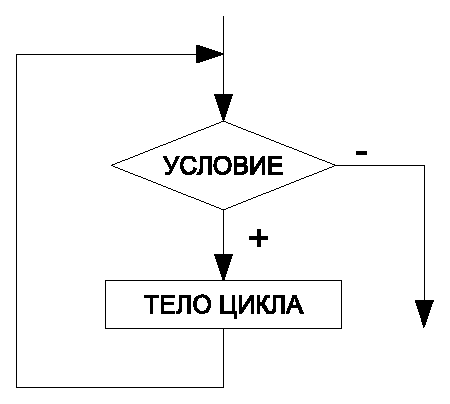
\includegraphics[width=0.3\textwidth]{img/ris_3_22}
\caption{Алгоритм циклической структуры с предусловием}
\label{ch03:refDrawing21}
\end{center}
\end{figure}

Работает цикл с предусловием следующим образом. Вычисляется \Sys{условие}. Если оно истинно (не равно
нулю), то выполняется \Sys{оператор}, и \Sys{условие} проверяется вновь. В противном случае цикл заканчивается, и управление передаётся
оператору, следующему за телом цикла. Условие вычисляется перед каждой итерацией цикла. Если при первой проверке
выражение равно нулю, цикл не выполнится ни разу. Тип выражения должен быть арифметическим или приводимым к нему. 

Если тело цикла состоит более чем из одного оператора, необходимо использовать составной оператор:
\begin{lstlisting}
while `\Sys{(условие)}`
{
  `\Sys{оператор 1;}`
  `\Sys{оператор 2;}`
  `\Sys{…}`
  `\Sys{оператор n;}`
}
\end{lstlisting}

Рассмотрим пример. Пусть необходимо вывести на экран таблицу значений функции  $y=e^{\sin (x)}\cos (x)$ на отрезке 
$[0;\pi]$ с шагом 0.1. Применив \emph{цикл с предусловием}, получим:
%\label{ch03:out0}
\begin{lstlisting}
#include <stdio.h>
#include <math.h>
#define PI 3.14159
using namespace std;
int main()
{
float x, y; //`Описание переменных`
x=0;        //`Присваивание параметру цикла стартового значения`
//`Цикл с предусловием`
while (x<=PI)	//`Пока параметр цикла не превышает конечное значение`
{ //`выполнять тело цикла`
  y=exp(sin(x))*cos(x); //`Вычислить значение` y
  //`Вывод на экран пары` x `и` y.
  printf("\t x=%5.2f \t y=%5.4f \n",x,y);
  x+=0.1;  //`Изменение параметра цикла` 
  //(`переход к следующему значению` x)
} //`Конец цикла`
return 0;
}
\end{lstlisting}

В результате работы данного фрагмента программы на экран последовательно будут выводиться сообщения со значениями
переменных $x$ и $y$\label{ch03:out0}:% (рис.~\ref{ch03:refDrawing22}).

\smallskip
\noindent%\begin{figure}[h]
\begin{minipage}{.3\textwidth}
\begin{verbatim}
x= 1.00      y=1.2534 
x= 1.10      y=1.1059 
x= 1.20      y=0.9203 
x= 1.30      y=0.7011 
x= 1.40      y=0.4553 
x= 1.50      y=0.1918 
x= 1.60      y=-0.0793 
x= 1.70      y=-0.3473 
x= 1.80      y=-0.6017 
x= 1.90      y=-0.8328 
x= 2.00      y=-1.0331
\end{verbatim}
\end{minipage}
%\hspace*{0.05\textwidth}
\begin{minipage}{.3\textwidth}
\begin{verbatim}
x= 2.10      y=-1.1969 
x= 2.20      y=-1.3209 
x= 2.30      y=-1.4045 
x= 2.40      y=-1.4489 
x= 2.50      y=-1.4576 
x= 2.60      y=-1.4348 
x= 2.70      y=-1.3862 
x= 2.80      y=-1.3172 
x= 2.90      y=-1.2334 
x= 3.00      y=-1.1400 
x= 3.10      y=-1.0416 
\end{verbatim}
\end{minipage}
\hfill
%\end{figure}

\subsection[Оператор цикла с постусловием]{Оператор цикла с постусловием}
В цикле с предусловием предварительной проверкой определяется, выполнять тело цикла или нет, до первой итерации. Если
это не соответствует логике алгоритма, то можно использовать \index{Оператор!цикл с постусловием}
\index{Алгоритм!цикл с постусловием}\emph{цикл с постусловием}. На рис.~\ref{ch03:refDrawing23}
видно, что в этом цикле проверяется, делать или нет очередную итерацию, лишь после завершения предыдущей. Это имеет
принципиальное значение лишь на первом шаге, а далее циклы ведут себя идентично. 

\begin{figure}[htb]
\begin{center}
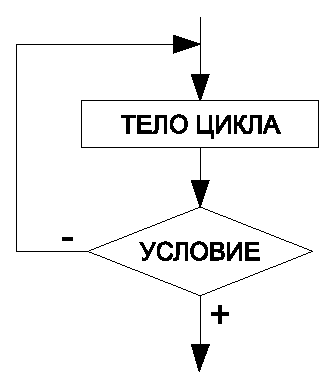
\includegraphics[width=0.3\textwidth]{img/ris_3_24}
\caption{Алгоритм циклической структуры с постусловием}
\label{ch03:refDrawing23}
\end{center}
\end{figure}

В \Sys{С++} \emph{цикл с постусловием} реализован конструкцией
\begin{lstlisting}
do `\Sys{оператор}` while `\Sys{(условие)}`;
\end{lstlisting}
здесь \Sys{условие} --- логическое или целочисленное выражение, 
\Sys{оператор} --- любой оператор языка С(С++). Если тело 
цикла состоит более чем из одного оператора:
\begin{lstlisting}
do
{
  `\Sys{оператор\_1;}`
  `\Sys{оператор\_2;}`
  `\Sys{…}`
  `\Sys{оператор\_n;}`
}
while `\Sys{(условие);}`
\end{lstlisting}

Работает цикл следующим образом. В начале выполняется оператор, представляющий собой тело цикла. Затем вычисляется
условие. Если оно истинно (не равно нулю), оператор тела цикла выполняется ещё раз. В противном случае цикл
завершается, и управление передаётся оператору, следующему за циклом.

Таким образом, не трудно заметить, что цикл с постусловием всегда будет выполнен хотя бы один раз, в отличие от цикла с
предусловием, который может не выполниться ни разу.

Если применить цикл с постусловием для создания программы, которая выводит таблицу 
значений функции  $y=e^{\sin (x)}\cos(x)$  на отрезке  $[0;\pi]$  с шагом 0.1, получим:

\begin{lstlisting}
#include <iostream>
#include <stdio.h>
#include <math.h>
#define PI 3.14159
using namespace std;
int main()
{
  float x, y;  //`Описание переменных`
  x=0; //`Присваивание параметру цикла стартового значения`
  do  //`Цикл с постусловием`
  {//`Выполнять тело цикла`
    y=exp(sin(x))*cos(x);
    printf(" \t x=%5.2f \t y=%5.4f \n",x,y);
    x+=0.1;  //`Изменение параметра цикла`
  }
  while(x<=PI);  //`пока параметр цикла не превышает конечное значение`
return 0;
}
\end{lstlisting}

Результаты работы этой программы будут такими же как на стр.~\pageref{ch03:out0}.%рис. \ref{ch03:refDrawing22}.

\subsection[Оператор цикла for с параметром]{Оператор цикла for с параметром}
Кроме того, в \Sys{С++} предусмотрен \index{Алгоритм!цикл с параметром}\index{Оператор!цикл с
параметром}\emph{цикл for с параметром}:
\begin{lstlisting}
for `\Sys{(начальные\_присваивания;условие;последействие)}`
`\Sys{оператор;}`
\end{lstlisting}
где \Sys{начальные\_присваивания} --- оператор или группа операторов, разделённых
запятой\footnote{Запятая в \Sys{С++} это операция последовательного выполнения операторов}, применяются для присвоения
начальных значений величинам, используемым в цикле, в том числе параметру цикла, и выполняются один раз в начале цикла;
\Sys{условие} --- целое или логическое выражение, которое определяет условие входа в цикл, если условие истинно (не равно
нулю), то цикл выполняется; \Sys{последействие} --- оператор или группа операторов, разделённых запятой,
которые выполняются после каждой итерации и служат для изменения параметра цикла; \Sys{оператор} --- любой
оператор языка, представляющий собой тело цикла. \Sys{Последействие} или \Sys{оператор}
должны влиять на условие, иначе цикл никогда не закончится. \Sys{Начальные\_присваивания},
\Sys{выражение} или \Sys{последействие} в записи оператора \Sys{for} могут
отсутствовать, но при этом «точки с запятой» должны оставаться на своих местах.

Опишем алгоритм работы цикла \Sys{for}:
\begin{enumerate}
\item Выполняются \Sys{начальные\_присваивания}.
\item Вычисляется \Sys{условие}, если оно не равно 0 (\Sys{true}), то выполняется переход к~п.3.
В противном случае выполнение цикла завершается.
\item Выполняется \Sys{оператор}. 
\item Выполняется оператор \Sys{последействие} и осуществляется переход к~п.2,  опять вычисляется значение
\Sys{выражения} и т.д.
\end{enumerate}
Понятно, что этот алгоритм представляет собой цикл с предусловием (рис.~\ref{ch03:refDrawing24}).
\begin{figure}[htb]
\begin{center}
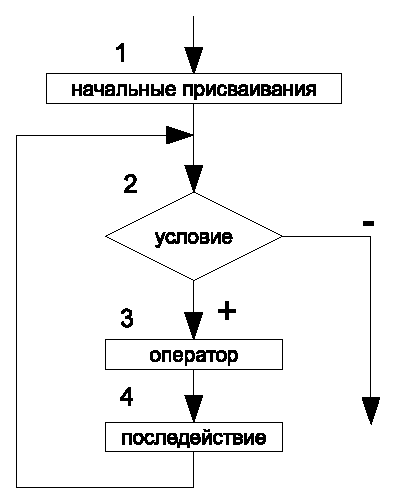
\includegraphics[width=0.3\textwidth]{img/ris_3_25}
\caption{Алгоритм работы цикла с параметром}
\label{ch03:refDrawing24}
\end{center}
\end{figure}

В дальнейшем, чтобы избежать создания слишком громоздких алгоритмов, в блок-схемах цикл \Sys{for} будем
изображать, так как показано на рис.~\ref{ch03:refDrawing25}.

В случае если тело цикла состоит более чем из одного оператора, необходимо использовать составной оператор:
\begin{lstlisting}
for `\Sys{(начальные\_присваивания; условие; последействие)}`
{
  `\Sys{оператор\_1;}`
  `\Sys{…}`
  `\Sys{оператор\_n;}`
}
\end{lstlisting}
Применение цикла \Sys{for} рассмотрим на примере печати таблицы значений функции  $y=e^{\sin (x)}\cos (x)$
на отрезке  $[0;\pi]$  с шагом 0.1:
\begin{figure}[htb]
\begin{center}
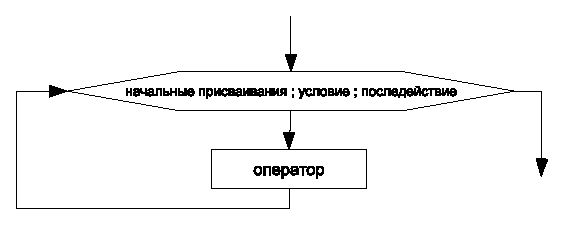
\includegraphics[width=0.5\textwidth]{img/ris_3_26}
\caption{Блок-схема цикла с параметром}
\label{ch03:refDrawing25}
\end{center}
\end{figure}

\begin{lstlisting}
#include <stdio.h>
#include <math.h>
#define PI 3.14159
using namespace std;
int main()
{
float x, y;
//`Параметру цикла присваивается начальное значение, если оно не превышает конечное значение,`
//`то выполняются операторы тела цикла и значение параметра изменяется, в противном случае`
//`цикл заканчивается.`
for (x=0;x<=PI;x+=0.1)
{
  y=exp(sin(x))*cos(x);
  printf("\t x=%5.2f \t y=%5.4f \n",x,y);
}
return 0;
}
\end{lstlisting}

Программный код выдаст результат, представленный на стр.~\pageref{ch03:out0}.% \ref{ch03:refDrawing22}.

\subsection[Операторы передачи управления]{Операторы передачи управления}
Операторы передачи управления принудительно изменяют порядок выполнения команд. В \Sys{С++} таких операторов четыре:
\Sys{goto}, \Sys{break}, \Sys{continue} и \Sys{return}.

Оператор \Sys{goto} \Sys{метка}, где \Sys{метка} обычный идентификатор, применяют
для безусловного перехода, он передаёт управление оператору с меткой: 
\Sys{метка: оператор};\footnote{Обычно применение оператора \Sys{goto} приводит к усложнению
программы и затрудняет отладку. Он нарушает принцип структурного программирования, согласно которому все блоки,
составляющие программу, должны иметь только один вход и один выход. В большинстве алгоритмов применения этого оператора
можно избежать}.

Оператор \Sys{break} осуществляет немедленный выход из циклов \Sys{while},
\Sys{do}…\Sys{while} и \Sys{for}, а так же из оператора выбора
\Sys{switch}. Управление передаётся оператору, находящемуся непосредственно за циклом или оператором
выбора. 

Оператор \Sys{continue} начинает новую итерацию цикла, даже если предыдущая не была завершена. 

Оператор \Sys{return} \Sys{выражение} завершает выполнение функции и передаёт управление в
точку её вызова. Если функция возвращает значение типа \Sys{void}, то выражение в записи оператора
отсутствует. В противном случае выражение должно иметь скалярный тип.

\section[Решение задач с использованием циклов]{Решение задач с использованием циклов}
Рассмотрим использование циклических операторов на конкретных примерах.

\prg{Написать программу решения квадратного уравнения
$ax^2+bx+c=0$. Предусмотреть проверку ввода данных.}{ch03:prg10}

Решение квадратного уравнения было подробно рассмотрено в задаче~\ref{ch03:prg4}. Однако алгоритм, изображённый 
на рис.~\ref{ch03:refDrawing14}, не будет работать, если пользователь введёт нулевое значение в переменную $a$ (при
попытке вычислить корни уравнения произойдёт деление на ноль). Чтобы избежать подобной ошибки нужно в программе
предусмотреть проверку входных данных, например, так как показано на рис.~\ref{ch03:refDrawing26}. 
Вводится значение переменной
$a$, если оно равно нулю, то ввод повторяется, иначе следует алгоритм вычисления корней квадратного
уравнения. Здесь применяется \emph{цикл с постусловием}, так как значение переменной необходимо ввести, а
затем проверить его на равенство нулю.

\begin{figure}[htb]
\begin{center}
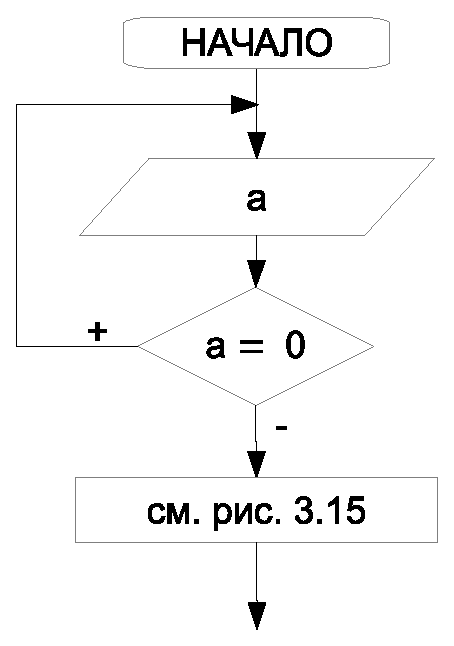
\includegraphics[width=0.3\textwidth]{img/ris_3_27}
\caption{Блок-схема проверки ввода данных}
\label{ch03:refDrawing26}
\end{center}
\end{figure}

Программа решения задачи:
\begin{lstlisting}
#include <iostream>
#include <math.h>
using namespace std;
int main()
{
float a,b,c,d,x1,x2;
//`Проверка ввода значения коэффициента` a.
do  //`Выполнять тело цикла пока а равно нулю`
{
  cout<<"a=";cin>>a;
}
while (a==0);
cout<<"b=";cin>>b;
cout<<"c=";cin>>c;
d=b*b-4*a*c;
if (d<0) cout<<"`Нет вещественных корней`";
else
{
x1=(-b+sqrt(d))/2/a;
x2=(-b-sqrt(d))/(2*a);
cout<<"X1="<<x1<<"\t X2="<<x2<<"\n";
}
return 0;
}
\end{lstlisting}

\prg{Найти наибольший общий делитель (НОД) натуральных чисел $A$
и $B$.}{ch03:prg11}

\emph{Входные данные}: $A$ и $B$.

\emph{Выходные данные}: $A$ --- НОД.

Для решения поставленной задачи воспользуемся алгоритмом Евклида: будем уменьшать каждый раз большее из чисел на
величину меньшего до тех пор, пока оба значения не станут равными, так, как показано в таблице~\ref{ch03:refTable1}. 


%%%%%%% Согласовать с авторами %%%%%%%%%
%{\tabcolsep=0.3em\noindent\small
%\begin{longtable}{|c|c|c|c|c|}
%\caption{Поиск НОД для чисел $A=25$ и $B=15$.} \label{ch03:refTable1}\\
%\hline
%\Emph{Исходные данные} & \Emph{Первый шаг} & \Emph{Второй шаг} & \Emph{Третий шаг} & \Emph{НОД(А,В)=5}\\
%\hline \hline
%\endfirsthead
%\multicolumn{5}{c}%
%{{\tablename\ \thetable{} --- продолжение}} \\
%\hline
%\Emph{Исходные данные} & \Emph{Первый шаг} & \Emph{Второй шаг} & \Emph{Третий шаг} & \Emph{НОД(А,В)=5}\\
%\hline \hline
%\endhead
%$A=25$ &$A=10$ &$A=10$ &$A=5$ &\\\hline
%$B=15$ &$B=15$ &$B=5$ &$B=5$ &\\\hline
%\end{longtable}
%}
%%%%%%%%%%%%%%%%%%%%%%%%%%%%%%%%
%{\tabcolsep=0.3em\noindent\small
\begin{longtable}{|l|c|c|}
\caption{Поиск НОД для чисел $A=25$ и $B=15$.} \label{ch03:refTable1}\\
\hline
\Emph{Шаг}&\Emph{A}&\Emph{B}\\
\hline\hline
\endfirsthead
\multicolumn{3}{c}%
{{\tablename\ \thetable{} --- продолжение}} \\
\hline
\Emph{Шаг}&\Emph{A}&\Emph{B}\\
\hline\hline
\endhead
Исходные данные&25&15\\\hline
Шаг 1&10&15\\\hline
Шаг 2&10&5\\\hline
Шаг 3, НОД&5&5\\\hline
\end{longtable}
%}
%%%%%%%%
%\begin{table}
%\begin{center}
%\caption{Поиск НОД для чисел $A=25$ и $B=15$.} \label{ch03:refTable1}
%\begin{tabular}{|l|c|c|}
%\hline
%\Emph{Шаг}&\Emph{A}&\Emph{B}\\
%\hline\hline
%Исходные данные&25&15\\\hline
%Шаг 1&10&15\\\hline
%Шаг 2&10&5\\\hline
%Шаг 3, НОД&5&5\\\hline
%\end{tabular}
%\end{center}
%\end{table}
%%%%%%%%%%%%

В блок–схеме, представленной на рис.~\ref{ch03:refDrawing27}, для решения поставленной задачи используется
\emph{цикл с предусловием}, то есть тело цикла повторяется до тех пор, пока $A$ не равно
$B$. Следовательно, при создании программы воспользуемся циклом \Sys{while}:

\begin{figure}[htb]
\begin{center}
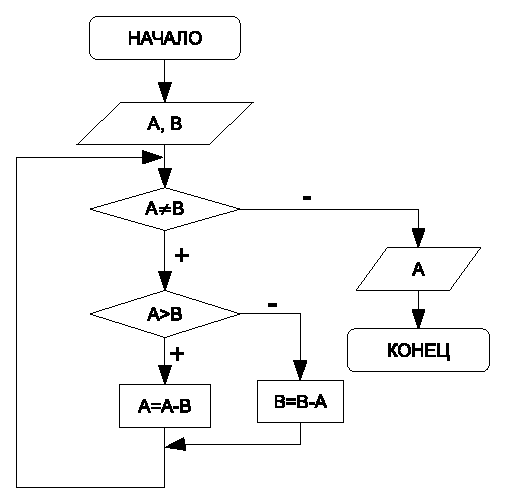
\includegraphics[width=0.5\textwidth]{img/ris_3_28}
\caption{Поиск наибольшего общего делителя двух чисел.}
\label{ch03:refDrawing27}
\end{center}
\end{figure}

\begin{lstlisting}
#include <iostream>
using namespace std;
int main()
{
  unsigned int a,b;
  cout<<"A="; cin>>a;
  cout<<"B="; cin>>b;
  //`Если числа не равны, выполнять тело цикла`
  while (a!=b)
  //`Если число` A `больше, чем` B, `то уменьшить его значение на` B,
    if (a>b) a=a-b;
  //`иначе уменьшить значение числа` B `на` A
    else b=b-a;
  cout<<"`НОД`="<<a<<"\n";
return 0;
}
\end{lstlisting}

Результат работы программы не изменится, если для её решения воспользоваться циклом с постусловием
\Sys{do…while}:

\begin{lstlisting}
#include <iostream>
using namespace std;
int main()
{
  unsigned int a,b;
  cout<<"A="; cin>>a;
  cout<<"B="; cin>>b;
  do
    if (a>b) a=a-b; else b=b-a;
  while (a!=b);
  cout<<"`НОД`="<<a<<"\n";
  return 0;
}
\end{lstlisting}

\prg{Вычислить факториал числа $N$ ( ${N}!=1\cdot 2\cdot 3\cdot \ldots \cdot N$).}{ch03:prg12}

\emph{Входные данные}: $N$ --- целое число, факториал которого необходимо вычислить.

\emph{Выходные данные}: \Sys{factorial} --- целое число, значение факториала числа $N$,
произведение чисел от 1 до $N$.

Промежуточные переменные: $i$ --- параметр цикла, целочисленная переменная, последовательно принимающая
значения 2, 3, 4 и так далее до $N$.

Блок-схема приведена на рис.~\ref{ch03:refDrawing28}.
\begin{figure}[htb]
\begin{center}
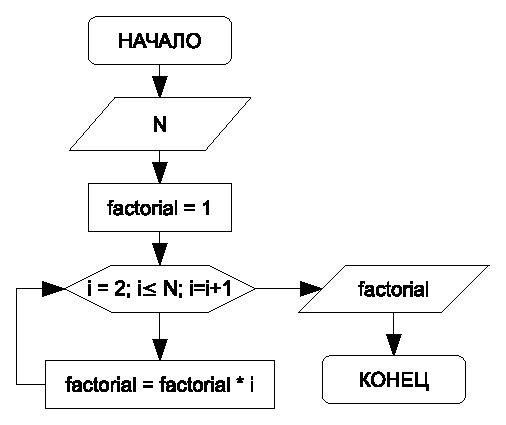
\includegraphics[width=0.5\textwidth]{img/ris_3_29}
\caption{Алгоритм вычисления факториала.}
\label{ch03:refDrawing28}
\end{center}
\end{figure}


Итак, вводится число $N$. Переменной \Sys{factorial}, предназначенной для хранения
значения произведения последовательности чисел, присваивается начальное значение, равное единице. Затем организуется
цикл, параметром которого выступает переменная $i$. Если значение параметра цикла не превышает
$N$, то выполняется оператор тела цикла, в котором из участка памяти с именем
\Sys{factorial} считывается предыдущее значение произведения, умножается на текущее значение параметра
цикла, а результат снова помещается в участок памяти с именем \Sys{factorial}. Когда параметр
$i$ превысит $N$, цикл заканчивается, и на экран выводится значение переменой
\Sys{factorial}, которая была вычислена в теле цикла.

Обратите внимание, как в программе записан \emph{оператор цикла}. Здесь операторы ввода и операторы
присваивания стартовых значений записаны как \Sys{начальные присваивания} цикла \Sys{for}, а
оператор накапливания произведения и оператор модификации параметра цикла представляют собой
\Sys{последействие}:
\begin{lstlisting}
#include <iostream>
using namespace std;
int main()
{
unsigned long long int factorial;1
unsigned int N, i;
for (cout<<"N=",cin>>N,factorial=1,i=2;i<=N;factorial*=i,i++);
cout<<"`факториал`="<<factorial<<"\n";
return 0;
}
\end{lstlisting}

\prg{Вычислить сумму натуральных чётных чисел, не превышающих~$N$.}{ch03:prg13}

\emph{Входные данные}: $N$ --- целое число.

\emph{Выходные данные}: $S$ --- сумма чётных чисел.

Промежуточные переменные: $i$ --- параметр цикла, принимает значения  2, 4, 6, 8 и так далее, также имеет
целочисленное значение.

При сложении нескольких чисел необходимо накапливать результат в определённом участке памяти (S), каждый раз считывая из
этого участка (S) предыдущее значение суммы (S) и прибавляя к нему слагаемое $i$. Для выполнения первого оператора
накапливания суммы из участка памяти необходимо взять такое число, которое не влияло бы на результат сложения. Перед
началом цикла переменной, предназначенной для накапливания сумы, необходимо присвоить значение нуль. Блок-схема решения
этой задачи представлена на рис.~\ref{ch03:refDrawing29}.

\begin{figure}[htb]
\begin{center}
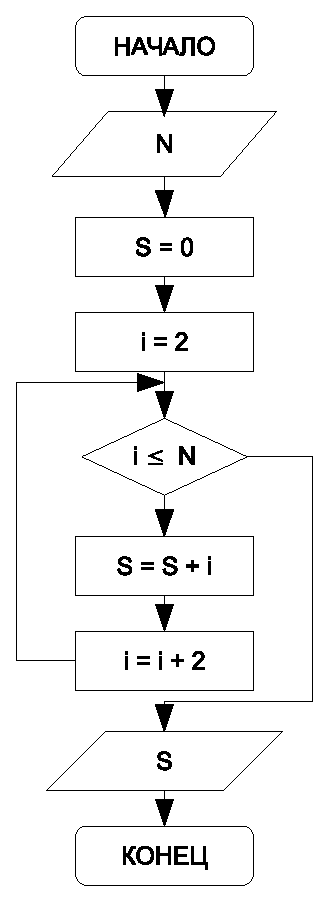
\includegraphics[width=0.3\textwidth]{img/ris_3_30}
\caption{Алгоритм вычисления суммы чётных натуральных чисел.}
\label{ch03:refDrawing29}
\end{center}
\end{figure}

Решим задачу двумя способами: с применением циклов \Sys{while} и \Sys{for}:

\begin{lstlisting}
//`Решение задачи с помощью цикла` while
#include <iostream>
using namespace std;
int main()
{
  unsigned int N,i,S;
  cout<<"N="; cin>>N;
  S=0;
  i=2;
  while (i<=N)
  {
    S=S+i;
    i=i+2;
  }
  cout<<"S="<<S<<"\n";
  return 0;
}
//----------------------------------
//`Решение задачи с помощью цикла` for
#include <iostream>
using namespace std;
int main()
{
  unsigned int N,i,S;
  for (cout<<"N=",cin>>N,S=0,i=2;i<=N;S+=i,i+=2);
    cout<<"S="<<S<<"\n";
  return 0;
}
\end{lstlisting}

\prg{Дано натуральное число $N$. Определить
$K$ --- количество делителей этого числа, меньших самого числа (Например, для $N$=12
делители 1, 2, 3, 4, 6. Количество $K$=5).}{ch03:prg14}

\emph{Входные данные}: $N$ --- целое число.

\emph{Выходные данные}: целое число $K$ --- количество делителей~$N$.

Промежуточные переменные: $i$ --- параметр цикла, возможные делители числа~$N$.

В блок-схеме, изображённой на рис.~\ref{ch03:refDrawing30}, реализован следующий алгоритм: в переменную $K$,
предназначенную для подсчёта количества делителей заданного числа, помещается значение, которое не влияло бы на
результат, т.е. нуль. Далее организовывается цикл, в котором изменяющийся параметр $i$ выполняет роль
возможных делителей числа $N$. Если заданное число $N$ делится нацело на параметр цикла $i$, это
означает, что $i$ является делителем $N$, и значение переменной $K$
следует увеличить на единицу. Цикл необходимо повторить $\frac{N}{2}$ раз.

\begin{figure}[htb]
\begin{center}
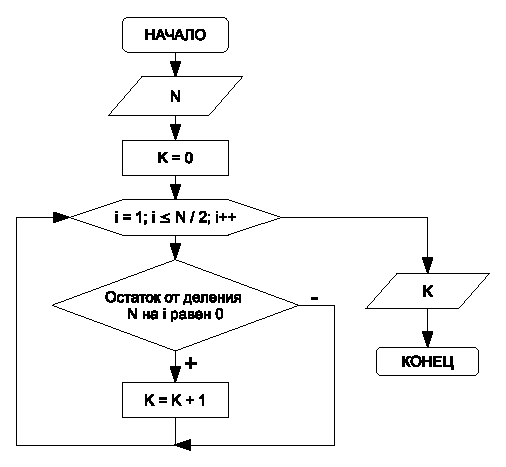
\includegraphics[width=0.8\textwidth]{img/ris_3_31}
\caption{Алгоритм определения делителей натурального числа.}
\label{ch03:refDrawing30}
\end{center}
\end{figure}

Текст программы на \Sys{С++}:
\begin{lstlisting}
#include <iostream>
using namespace std;
int main()
{
  unsigned int N,i,K;
  cout<<"N="; cin>>N;
  for (K=0,i=1;i<=N/2;i++) if (N%i==0) K++;
  cout<<"K="<<K<<"\n";
  return 0;
}
\end{lstlisting}

\prg{Дано натуральное число $N$.
Определить, является ли оно простым. Натуральное число $N$ называется простым, если оно делится без
остатка только на единицу и на само себя. Число 13 --- простое, так как делится только на 1 и 13, а число 12 таковым не
является, так как делится на 1, 2, 3, 4, 6 и 12.}{ch03:prg15}

\emph{Входные данные}: $N$ --- целое число.

\emph{Выходные данные}: сообщение.

Промежуточные переменные: $i$ --- параметр цикла, возможные делители числа~$N$.

Необходимо проверить, есть ли делители числа $N$ в диапазоне от $2$ до $N/2$ (рис.~\ref{ch03:refDrawing31}). Если
делителей нет, $N$ --- простое число, иначе оно таковым не является. Обратите внимание на то, что в
алгоритме предусмотрено два выхода из цикла. Первый --- естественный, при исчерпании всех значений параметра, 
а второй --- досрочный. Нет смысла продолжать цикл, если будет найден хотя бы один  делитель из указанной области изменения
параметра.

\begin{figure}[htb]
\begin{center}
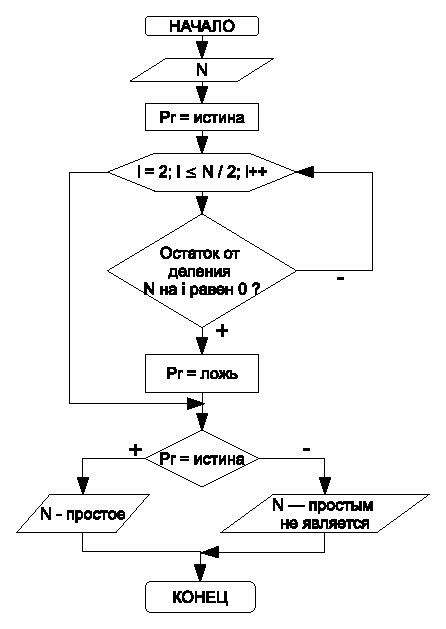
\includegraphics[width=0.5\textwidth]{img/ris_3_32}
\caption{Алгоритм определения простого числа.}
\label{ch03:refDrawing31}
\end{center}
\end{figure}

При составлении программы на языке \Sys{С++} досрочный выход из цикла удобно выполнять при помощи оператора
\Sys{break}:
\begin{lstlisting}
#include <iostream>
using namespace std;
int main()
{
unsigned int N,i;
bool Pr;
cout<<"N="; cin>>N;
Pr=true;  //`Предположим, что число простое`
for (i=2;i<=N/2;i++)
  if (N%i==0) //`Если найдётся хотя бы один делитель, то`
  {
    Pr=false; //`число простым не является и`
    break; //`досрочный выход из цикла`
  }
  if (Pr) //`Проверка значения логического параметра и вывод на печать`
          //`соответствующего сообщения`
    cout<<N<<" - `\Sys{простое число}`\n";
  else
    cout<<N<<" - `\Sys{не является простым}`\n";
return 0;
}
\end{lstlisting}

\prg{Дано натуральное число $N$. Определить количество цифр в числе.}{ch03:prg16}

\emph{Входные данные}: $N$ --- целое число.

\emph{Выходные данные}: $kol$ --- количество цифр в числе.

\emph{Промежуточные данные}: $M$ --- переменная для временного хранения значения
$N$\footnote{При решении задачи (см. алгоритм на рис.~\ref{ch03:refDrawing32}) исходное число изменятся,
поэтому, чтобы его, не потерять, копируем исходное число $N$ в переменную $M$, и делить будем уже $M$.}.

Для того, чтобы подсчитать количество цифр в числе, необходимо определить, сколько раз заданное число можно разделить на
десять нацело. Например, пусть $N=12345$, тогда количество цифр $kol = 5$. Результаты
вычислений сведены в таблицу \ref{ch03:refTable2}.

\begin{longtable}{|c|c|}
\caption{Определение количества цифр числа} \label{ch03:refTable2}\\
\hline
\Emph{kol} & \Emph{N}\\
\hline \hline
\endfirsthead
\multicolumn{2}{c}%
{{\tablename\ \thetable{} --- продолжение}} \\
\hline
\Emph{kol} & \Emph{N}\\
\hline \hline
\endhead
1 & 12345\\\hline
2 & 12345 / 10 = 1234\\\hline
3 & 1234 / 10 = 123\\\hline
4 & 123 / 10 = 12\\\hline
5 & 12 / 10 = 1\\\hline
 & 1 / 10 = 0\\\hline
\end{longtable}

Алгоритм определения количества цифр в числе представлен на рис.~\ref{ch03:refDrawing32}.

\begin{figure}[htb]
\begin{center}
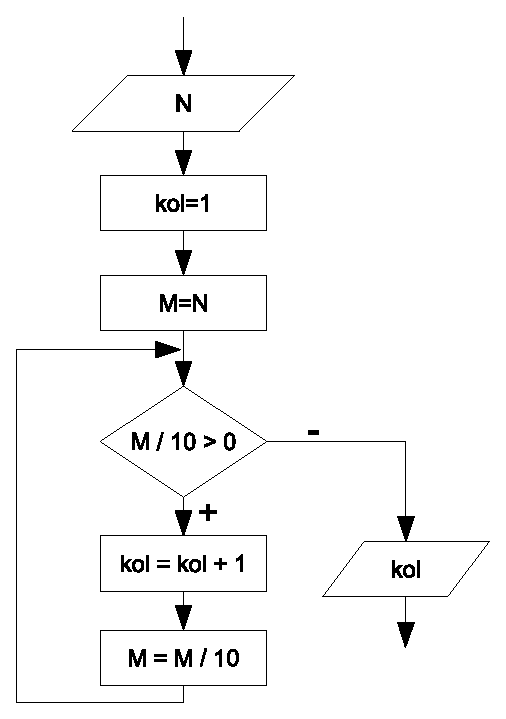
\includegraphics[width=0.5\textwidth]{img/ris_3_33}
\caption{Алгоритм определения количества цифр в числе.}
\label{ch03:refDrawing32}
\end{center}
\end{figure}

\begin{lstlisting}
#include <iostream>
using namespace std;
int main()
{
	unsigned long int N, M;
	unsigned int kol;
	cout<<"N="; cin>>N;
	for (M=N, kol=1; M/10>0; kol++,M/=10);
	cout<<"kol="<<kol<<endl;
return 0;
}
\end{lstlisting}

\prg{Дано натуральное число $N$. Определить,
содержит ли это число нули и в каких разрядах они расположены (например, число 11011110111 содержит ноль в третьем и
восьмом разрядах, а число 120405 ---  в первом и третьем).}{ch03:prg17}

\emph{Входные данные}: $N$ --- целое число. 

\emph{Выходные данные}: $pos$ --- позиция цифры в числе. 

\emph{Промежуточные данные}: $i$ --- параметр цикла, $M$ --- переменная для
временного хранения значения $N$.

В связи с тем, что разряды в числе выделяются начиная с последнего, для определения номера разряда в числе,
необходимо знать количество цифр в числе\footnote{Алгоритм нахождения количества цифр в числе был рассмотрен в
предыдущей задаче.}. Таким образом, на первом этапе решения задачи необходимо определить $kol$ ---
количество цифр в числе. Затем нужно выделять из числа цифры, если очередная цифра равна нулю, вывести на экран номер
разряда, который занимает эта цифра. Процесс определения текущей цифры числа
$N=120405$ представлен в таблице~\ref{ch03:refTable3}.

\begin{longtable}{|c|l|l|c|}
\caption{Определение текущей цифры числа} \label{ch03:refTable3}\\
\hline
\Emph{i} & \Emph{Число М} & \Emph{Цифра} & \Emph{Номер позиции}\\
\hline \hline
\endfirsthead
\multicolumn{4}{c}%
{{\tablename\ \thetable{} --- продолжение}} \\
\hline
\Emph{i} & \Emph{Число М} & \Emph{Цифра} & \Emph{Номер позиции}\\
\hline \hline
\endhead
1 & 120405 & 120405 \% 10 = 5 &0\\\hline
2 & 12040/10 = 1204 & 12040 \% 10 = 0 & \Emph{1}\\\hline
3 & 1204/10 = 120 & 1204 \% 10 = 4 & 2\\\hline
4 & 120/10 = 12 & 120 \% 10 = 0 & \Emph{3}\\\hline
5 & 12/10 = 1 & 12 \% 10 = 2 & 4\\\hline
6 & 1/10 = 0 & 1 \% 10 = 1 & 5\\\hline
\end{longtable}

Программный код к задаче~\ref{ch03:prg17}.
\begin{lstlisting}
#include <iostream>
using namespace std;
int main()
{
  unsigned long int N,M; int kol, i;
  cout<<"N="; cin>>N;
  for (kol=1,M=N;M/10>0; kol++,M/=10);
    for (M=N,i=0;i<kol;M/=10,i++)
      if (M%10==0) cout<<"`\Sys{Позиция}` = "<<i<<endl;
  return 0;
}
\end{lstlisting}

\prg{Дано натуральное число $N$. Получить
новое число, записав цифры числа $N$ в обратном порядке. Например, 17852 --- 25871.}{ch03:prg18}

\emph{Входные данные}: $N$ --- целое число.

\emph{Выходные данные}: $S$ --- целое число, полученное из цифр числа $N$, записанных в обратном порядке.

\emph{Промежуточные данные}: $i$ --- параметр цикла, $M$ --- переменная для
временного хранения значения $N$, $kol$ --- количество разрядов в заданном числе, 
$R=10^{kol}$ --- старший разряд заданного числа.

Рассмотрим пример. Пусть $N=17852$, тогда 
$S=2\cdot 10^4+5\cdot 10^3+8\cdot 10^2+7\cdot 10^1+1\cdot 10^0=25871$.

Значит, для решения поставленной задачи, нужно знать количество
разрядов в заданном числе $kol$ и его старший разряд $R=10^{kol}$.
Новое число $S$ формируют как сумму произведений
последней цифры заданного числа на старший разряд $S+=M\%10*R$. Цикл выполняют
$kol$ раз, при каждой итерации уменьшая само число и старший разряд в десять раз.
\begin{lstlisting}
#include <iostream>
using namespace std;
int main()
{unsigned long int N,M,R,S; int kol, i;
cout<<"N="; cin>>N;
for (R=1,kol=1,M=N;M/10>0; kol++,R*=10,M/=10);
  for(S=0,M=N,i=1;i<=kol;S+=M%10*R,M/=10,R/=10,i++);
    cout<<"S="<<S<<endl;
return 0;
}
\end{lstlisting}

\prg{Проверить, является ли заданное число $N$ палиндромом\protect\footnotemark . 
Например, числа 404, 1221 --- палиндромы.}{ch03:prg19}%
\footnotetext{
Палиндром --- это число, слово или фраза одинаково читающееся в обоих направлениях, или, другими
словами, любой симметричный относительно своей середины набор символов.
}

\emph{Входные данные}: $N$ --- целое число.

\emph{Выходные данные}: \Sys{сообщение}. 

\emph{Промежуточные данные}: $i$ --- параметр цикла, $M$ --- переменная для
временного хранения значения $N$, $kol$ --- количество разрядов в заданном числе,
$R=10^{kol}$ --- старший разряд заданного числа, $S$ --- целое число, полученное 
из цифр числа $N$, записанных в обратном порядке.

Можно предложить следующий алгоритм решения задачи. Записать цифры заданного числа $N$ в обратном
порядке (задача~\ref{ch03:prg18}), получится новое число $S$.
Сравнить полученное число $S$ с исходным $N$. Если числа равны,
то заданное число является палиндромом.

Текст программы на языке \Sys{С++}:
\begin{lstlisting}
#include <iostream>
using namespace std;
int main()
{unsigned long int N,M,R,S; 
int kol, i;
cout<<"N="; cin>>N;
for (R=1,kol=1,M=N;M/10>0; kol++,R*=10,M/=10);
  for(S=0,M=N,i=1;i<=kol;S+=M%10*R,M/=10,R/=10,i++);
    if (N==S) cout<<"`\Sys{Число - палинром}`"<<endl;
    else cout<<"`\Sys{Число не является палиндромом}`"<<endl;
return 0;
}
\end{lstlisting}


\prg{Поступает последовательность из $N$ вещественных чисел.
Определить наибольший элемент последовательности.}{ch03:prg20}

\emph{Входные данные}: $N$ --- целое число; $X$ --- вещественное число,
определяет текущий элемент последовательности.

\emph{Выходные данные}: $Max$ --- вещественное число, элемент последовательности с
наибольшим значением.

\emph{Промежуточные переменные}: $i$ --- параметр цикла, номер вводимого элемента
последовательности.

Алгоритм поиска наибольшего элемента в последовательности следующий (рис.~\ref{ch03:refDrawing33}). 
Вводится $N$ --- количество элементов последовательности и $X$ --- первый элемент последовательности. 
В памяти компьютера отводится ячейка, например с
именем $Max$, в которой будет храниться наибольший элемент последовательности --- максимум. Далее
предполагаем, что первый элемент последовательности наибольший и записываем его в $Max$. Затем
вводим второй элемент последовательности и сравниваем его с предполагаемым максимумом. Если окажется, что второй
элемент больше, его записывают в ячейку $Max$. В противном случае никаких действий не предпринимаем.
Потом переходим к вводу следующего элемента последовательности ($X$), и алгоритм повторяется с начала. В результате в
ячейке $Max$ сохранится элемент последовательности с наибольшим значением\footnote{Для поиска
наименьшего элемента последовательности (минимума), предполагают, что первый элемент --- наименьший, записывают его в
ячейку $min$, а затем среди элементов последовательности ищут число, значение которого будет меньше чем предполагаемый
минимум.}.

\begin{figure}[htb]
\begin{center}
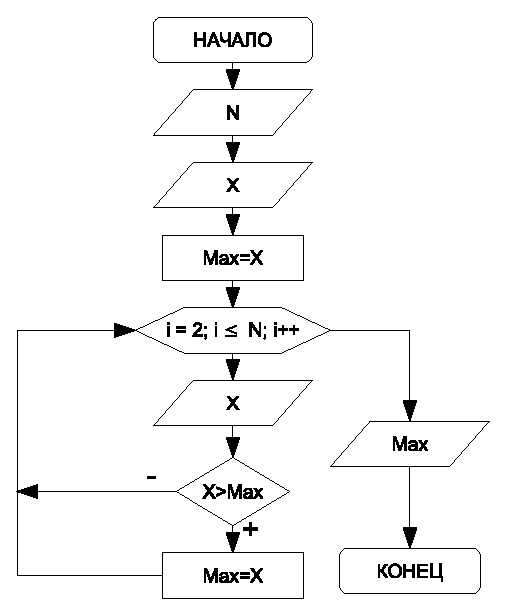
\includegraphics[width=0.5\textwidth]{img/ris_3_34}
\caption{Алгоритм поиска наибольшего числа в последовательности.}
\label{ch03:refDrawing33}
\end{center}
\end{figure}

Текст программы на \Sys{С++}:
\begin{lstlisting}
#include <iostream>
using namespace std;
int main()
{
  unsigned int i,N;
  float X,Max;
  cout<<"N="; cin>>N;
  cout<<"X="; cin>>X; //`Ввод первого элемента последовательности`
  //`Параметр цикла принимает стартовое значение` i=2, `т.к. первый элемент`
  //`уже введён предположим, что он максимальный, т.е.` Max=X.
  for (i=2, Max=X; i<=N;i++)
  {
    cout<<"X="; cin>>X; //`Ввод следующих элементов последовательности.`
  //`Если найдётся элемент, превышающий максимум, записать его в ячейку` Max, 
  //`теперь он предполагаемый максимум.`
  if (X>Max) Max=X;
  }
  //`Вывод наибольшего элемента последовательности.`
  cout<<"Max="<<Max<<"\n";
  return 0;
}
\end{lstlisting}

\prg{Вводится последовательность целых чисел, 0 --- конец последовательности. Найти
наименьшее число среди положительных, если таких значений несколько\protect\footnote{Предположим вводится последовательность
чисел 11, -3, 5, 12, -7, 5, 8,-9, 7, -6, 10, 5, 0. Наименьшим положительным числом является 5. Таких минимумов в
последовательности 3.}, определить, сколько их.}{ch03:prg21}

%\footnote{
%Предположим вводится последовательность
%чисел 11, -3, 5, 12, -7, 5, 8,-9, 7, -6, 10, 5,0. Наименьшим положительным числом является 5. Таких минимумов в
%последовательности 3.
%}

Блок-схема решения задачи приведена на рис. \ref{ch03:refDrawing34}.
\begin{figure}[htb]
\begin{center}
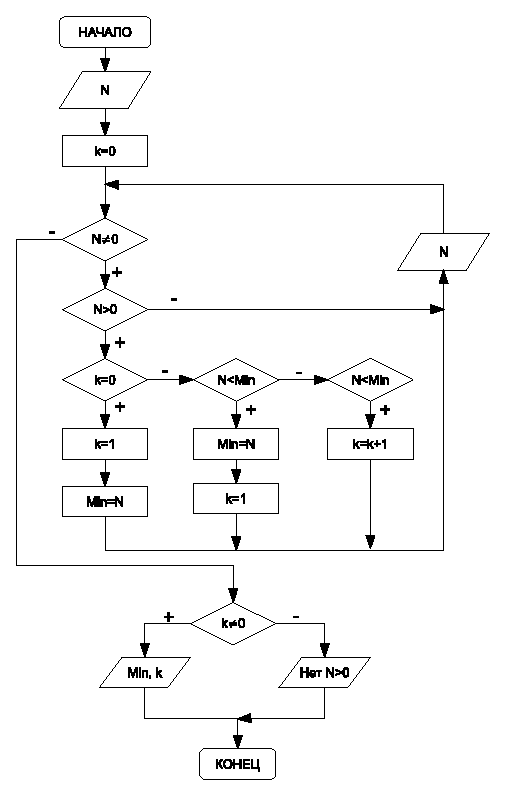
\includegraphics[width=0.8\textwidth]{img/ris_3_35}
\caption{Алгоритм поиска минимального положительного числа в последовательности.}
\label{ch03:refDrawing34}
\end{center}
\end{figure}

Далее приведён текст подпрограммы с подробными комментариями\footnote{Алгоритм поиска максимального (минимального)
элементов последовательности подробно описан в задаче~\ref{ch03:prg20}}.

\begin{lstlisting}
#include <iostream>
using namespace std;
int main()
{
  float N,Min; int K;
  //`Предположим, что в последовательности нет положительных чисел`, K=0.
  //`Вводим число и если оно не равно нулю`
  for (cout<<"N=",cin>>N,K=0;N!=0;cout<<"N=",cin>>N)
    //`проверяем является ли оно положительным.`
    if (N>0)
      //`если K=0, поступил 1-й положительный элемент, предположим, что он минимальный.`
      if (K==0) {K=1;Min=N;}
        //`если элемент не первый, сравниваем его с предполагаемым минимумом,`
        //`если элемент меньше, записываем его в` Min `и сбрасываем счётчик`
      else if (N<Min) {Min=N;K=1;}
           //`если элемент равен минимуму, увеличиваем значение счётчика.`
           else if (N==Min) K++; //`Конец цикла`
  //`Если значение счётчика не равно нулю, печатаем значение`
  //`минимального элемента и количество таких элементов.`
  if (K!=0) cout<<"Min="<<Min<<"\n"<<"K="<<K<<"\n";
  //`в противном случае выдаём сообщаем.`
  else cout<<"`\Sys{В последовательности нет положительных элементов}` \n";
  return 0;
}
\end{lstlisting}


\prg{Определить, сколько раз последовательность из
$N$ произвольных чисел меняет знак.}{ch03:prg22}

Чтобы решить задачу, нужно попарно перемножать элементы последовательности. Если результат произведения пары чисел ---
отрицательное число, значит, эти числа имеют разные знаки. 

Пусть в переменной $B$ хранится текущий элемент последовательности, в $A$ --- предыдущий. Введём первое 
число $A$ (до цикла) и
второе $B$ (в цикле). Если их произведение отрицательно, то увеличиваем количество смен знака на 1 (\Sys{k++}). После чего
сохраняем значение $B$ в переменную $A$ и повторяем цикл (рис.~\ref{ch03:refDrawing35}).

\begin{figure}[htb]
\begin{center}
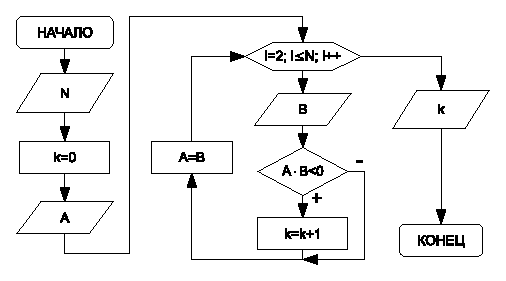
\includegraphics[width=0.6\textwidth]{img/ris_3_36}
\caption{Алгоритм решения задачи~\ref{ch03:prg22}.}
\label{ch03:refDrawing35}
\end{center}
\end{figure}

Предлагаем читателю самостоятельно разобраться с текстом программы на \Sys{С++}: 
\begin{lstlisting}
#include <iostream>
using namespace std;
int main()
{
  float A,B; int i,K,N;
  cout<<"N=";cin>>N;
  for (K=0,cout<<"A=",cin>>A,i=2;i<=N;i++)
  {
    cout<<"B=";cin>>B;
    if (A*B<0) K++;
    A=B;
  }
  cout<<"K="<<K<<"\n";
  return 0;
}
\end{lstlisting}


\prg{Поступает последовательность из $N$ вещественных чисел. Определить количество
простых чисел в последовательности.}{ch03:prg23}

Блок-схема алгоритма изображена на рис.~\ref{ch03:refDrawing36}. Обратите внимание, что для решения задачи было организовано два
цикла. Первый цикл обеспечивает ввод элементов последовательности. Второй цикл находится внутри первого и определяет,
является ли поступившее число простым (задача~\ref{ch03:prg15}).

\begin{figure}[htb]
\begin{center}
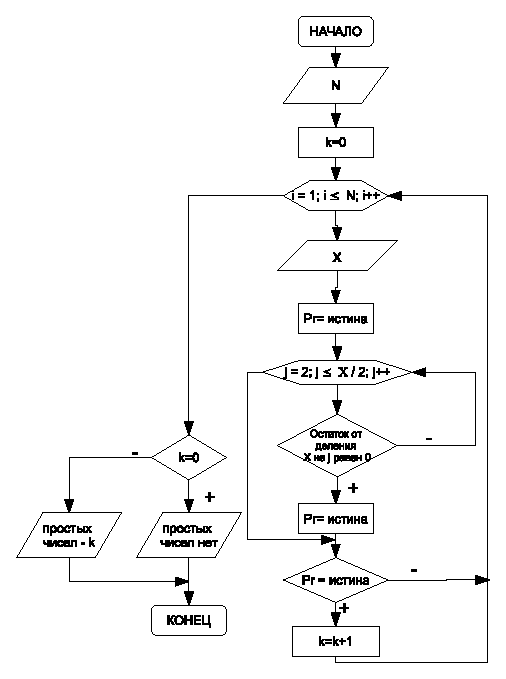
\includegraphics[width=0.5\textwidth]{img/ris_3_37}
\caption{Алгоритм поиска простых чисел в последовательности.}
\label{ch03:refDrawing36}
\end{center}
\end{figure}

\begin{lstlisting}
#include <iostream>
using namespace std;
int main()
{
  unsigned long int X; 
  unsigned int N; 
  int i,k,j;
  bool Pr;
  for (k=0,cout<<"N=", cin>>N, i=1;i<=N;i++)
  {
    for (cout<<"X=", cin>>X,Pr=true,j=2;j<=X/2;j++)
      if (X%j==0) 
      {
        Pr=false;
        break;
      }
      if (Pr) k++;
  }
  if (k==0) cout<<"`\Sys{Простых чисел нет}` \n";
  else  cout<<"`\Sys{Количество простых чисел}` k="<<k<<"\n";
return 0;
}
\end{lstlisting}

\prg{Дано $K$ наборов ненулевых целых чисел. Каждый набор
содержит не менее двух элементов, признаком его завершения является число 0. Найти количество наборов, элементы которых
возрастают.}{ch03:prg24}

Блок-схема алгоритма решения задачи показана на рис.~\ref{ch03:refDrawing37}. Нетрудно заметить, что алгоритм реализован с
помощью двух циклических процессов. Внутренний цикл проверяет является ли последовательность возрастающей, а внешний
повторяет алгоритм для новой последовательности.

\begin{figure}[htb]
\begin{center}
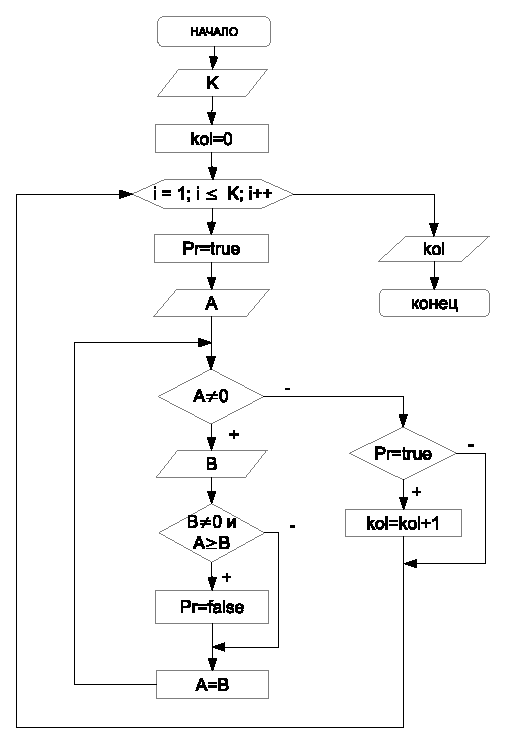
\includegraphics[width=0.6\textwidth]{img/ris_3_38}
\caption{Алгоритм решения задачи~\ref{ch03:prg24}.}
\label{ch03:refDrawing37}
\end{center}
\end{figure}

Программный код решения задачи~\ref{ch03:prg24}:
\begin{lstlisting}
#include <iostream>
using namespace std;
int main()
{
  unsigned int K, i,kol, A, B; bool pr;
  for (cout<<"K=", cin>>K, kol=0,i=1;i<=K;i++)
  {
    for (pr=true,cout<<"A=",cin>>A;A!=0; A=B)
    {
      cout<<"B="; cin>>B;
      if (B!=0 && A>=B) pr=false;
    }
    if (pr) kol++;
  }
  cout << "kol=" << kol<<endl;
  return 0;
}
\end{lstlisting}


\section[Задачи для самостоятельного решения]{Задачи для самостоятельного решения}
\subsection[Разветвляющийся процесс. Вычисление значения функции.]{Разветвляющийся процесс. Вычисление значения
функции.}
Разработать программу на языке \Sys{С++}. Дано вещественное число $a$. Для функции
$y=f(x)$, график которой приведён ниже, вычислить
$f(a)$. Варианты заданий представлены на рис.~\ref{ch03:refDrawing38}--\ref{ch03:refDrawing62}.

%%%%%% рис 39, 40 и 41 в ряд 
\floatsetup[widefloat]{margins=hangleft}
\begin{figure}[h]%
\begin{floatrow}[3]
\ffigbox[\FBwidth]
{\caption{Задание~1}%
\label{ch03:refDrawing38}}
{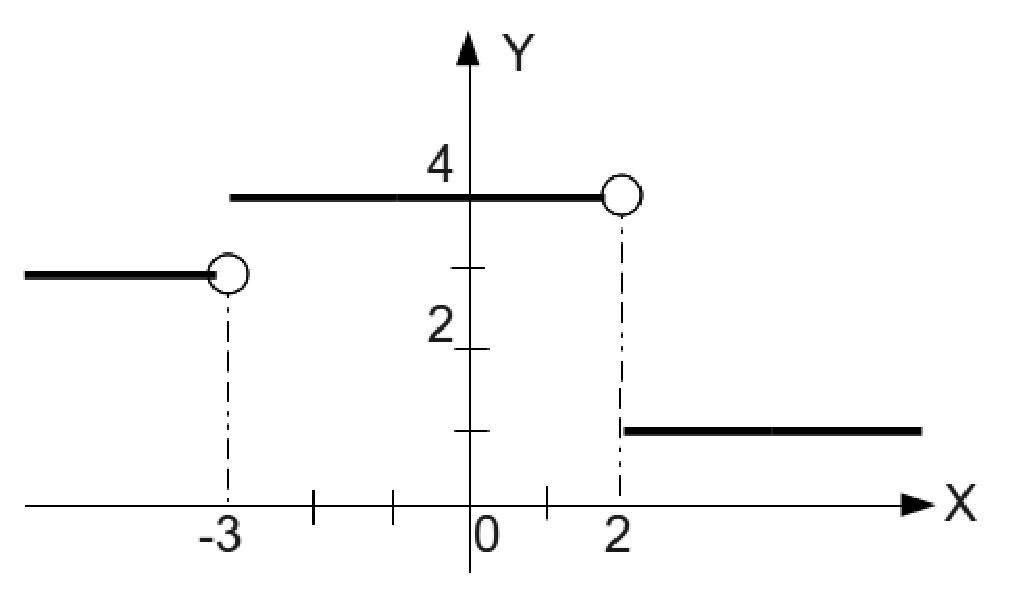
\includegraphics[width=0.32\textwidth,keepaspectratio]{img/ris_3_39}}
\ffigbox[\FBwidth]
{\caption{Задание~2}%
\label{ch03:refDrawing39}}
{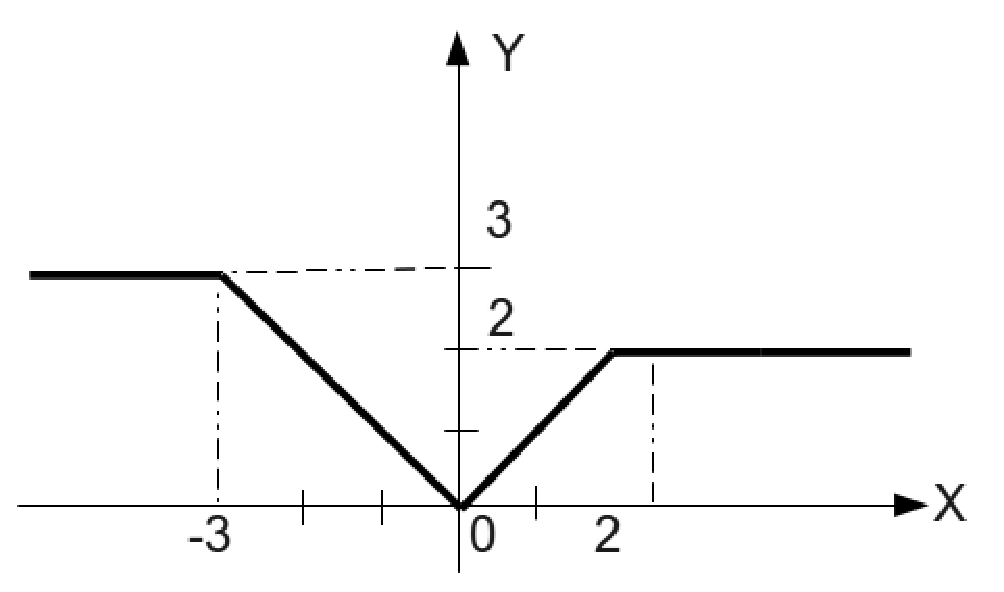
\includegraphics[width=0.32\textwidth,keepaspectratio]{img/ris_3_40}}
\ffigbox[\FBwidth]
{\caption{Задание~3}%
\label{ch03:refDrawing40}}
{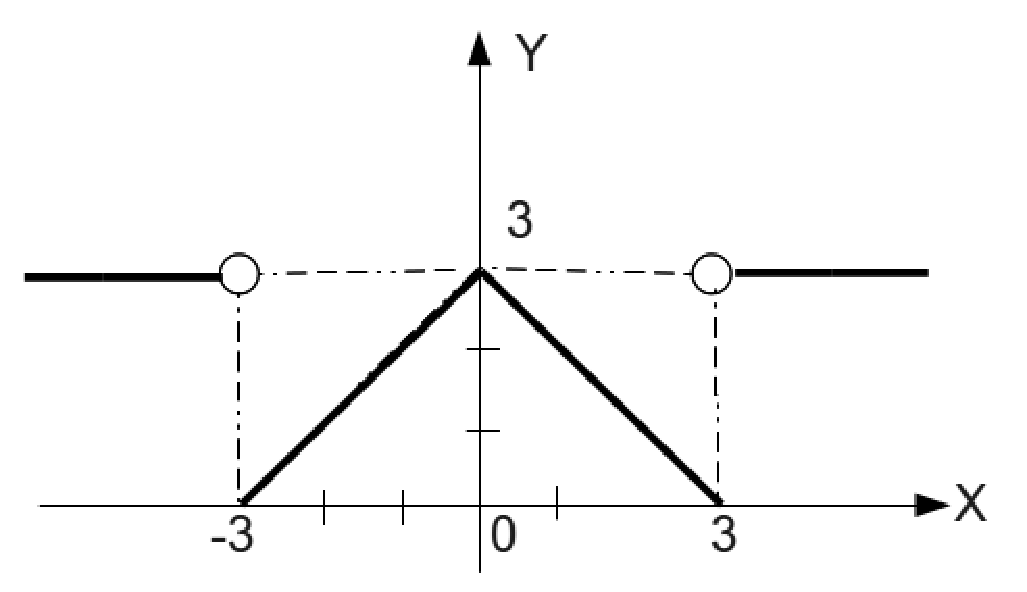
\includegraphics[width=0.32\textwidth,keepaspectratio]{img/ris_3_41}}
\end{floatrow}
\end{figure}%
%%%% end 39, 40, 41

%%%%%% рис 42, 43 и 44 в ряд 
\floatsetup[widefloat]{margins=hangleft}
\begin{figure}[h]%
\begin{floatrow}[3]
\ffigbox[\FBwidth]
{\caption{Задание~4}%
\label{ch03:refDrawing41}}
{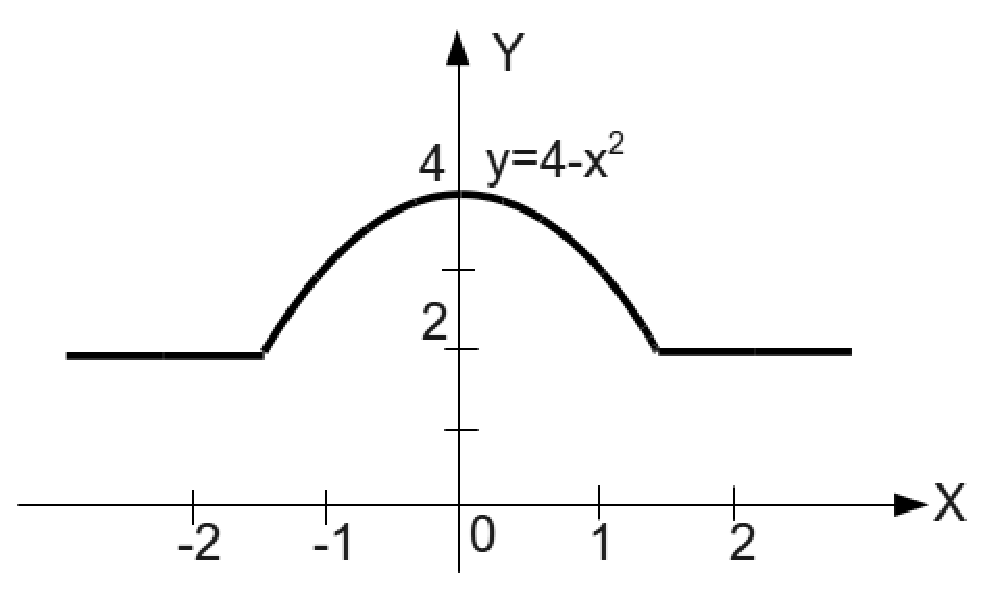
\includegraphics[width=0.32\textwidth,keepaspectratio]{img/ris_3_42}}
\ffigbox[\FBwidth]
{\caption{Задание~5}%
\label{ch03:refDrawing42}}
{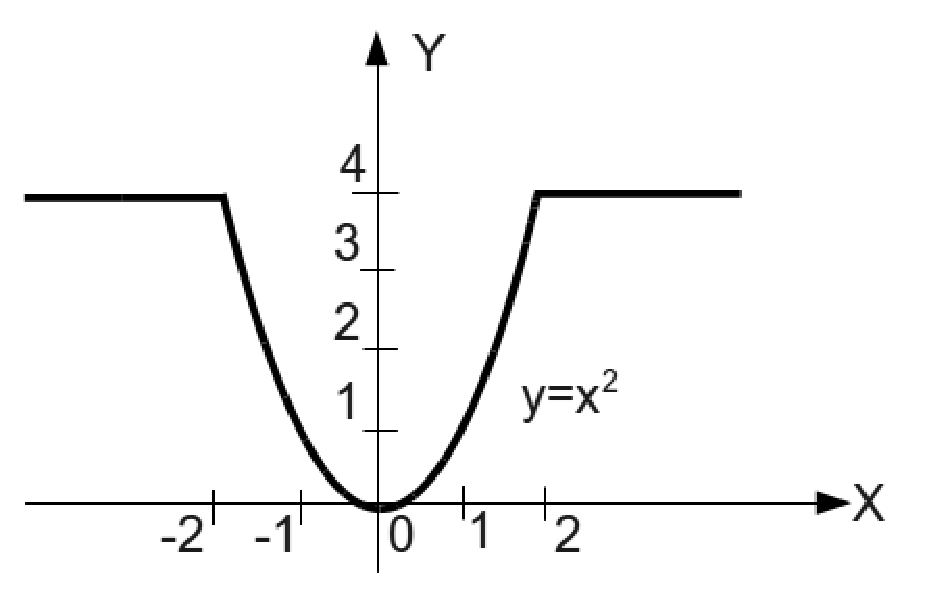
\includegraphics[width=0.32\textwidth,keepaspectratio]{img/ris_3_43}}
\ffigbox[\FBwidth]
{\caption{Задание~6}%
\label{ch03:refDrawing43}}
{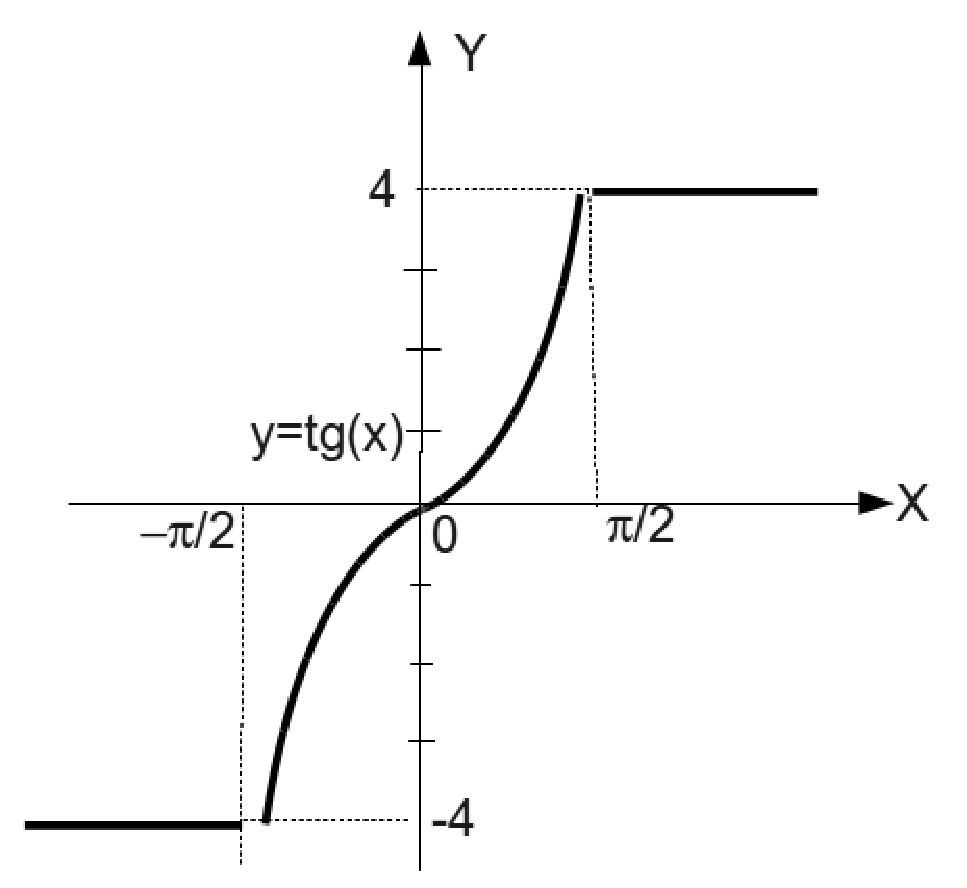
\includegraphics[width=0.32\textwidth,keepaspectratio]{img/ris_3_44}}
\end{floatrow}
\end{figure}%
%%%% end 42, 43, 44

%%%%%% рис 45, 46 и 47 в ряд 
\floatsetup[widefloat]{margins=hangleft}
\begin{figure}%
\begin{floatrow}[3]
\ffigbox[\FBwidth]
{\caption{Задание~7}%
\label{ch03:refDrawing44}}
{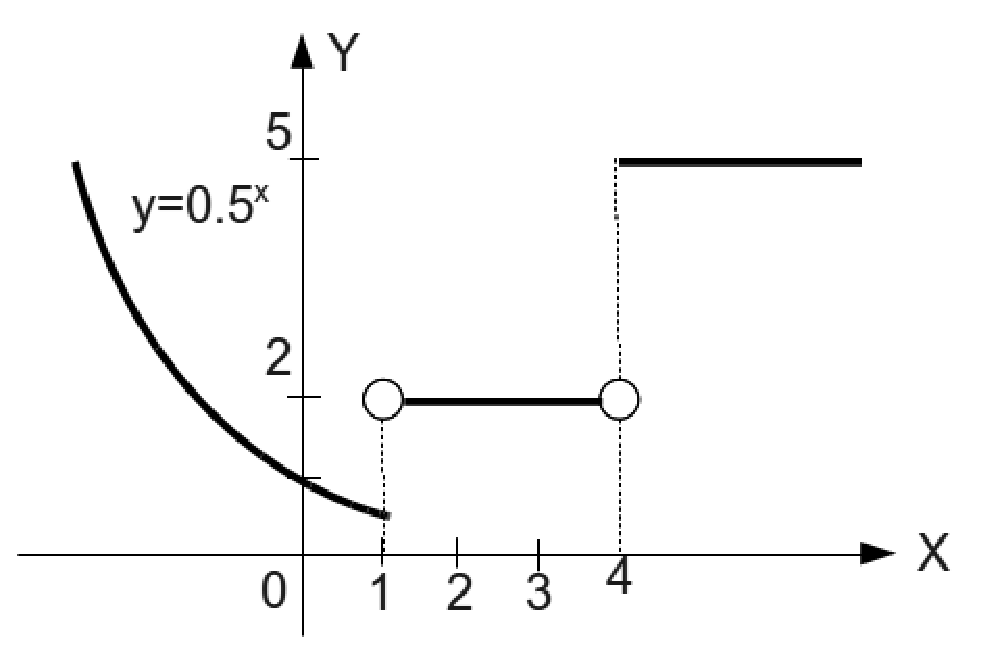
\includegraphics[width=0.32\textwidth,keepaspectratio]{img/ris_3_45}}
\ffigbox[\FBwidth]
{\caption{Задание~8}%
\label{ch03:refDrawing45}}
{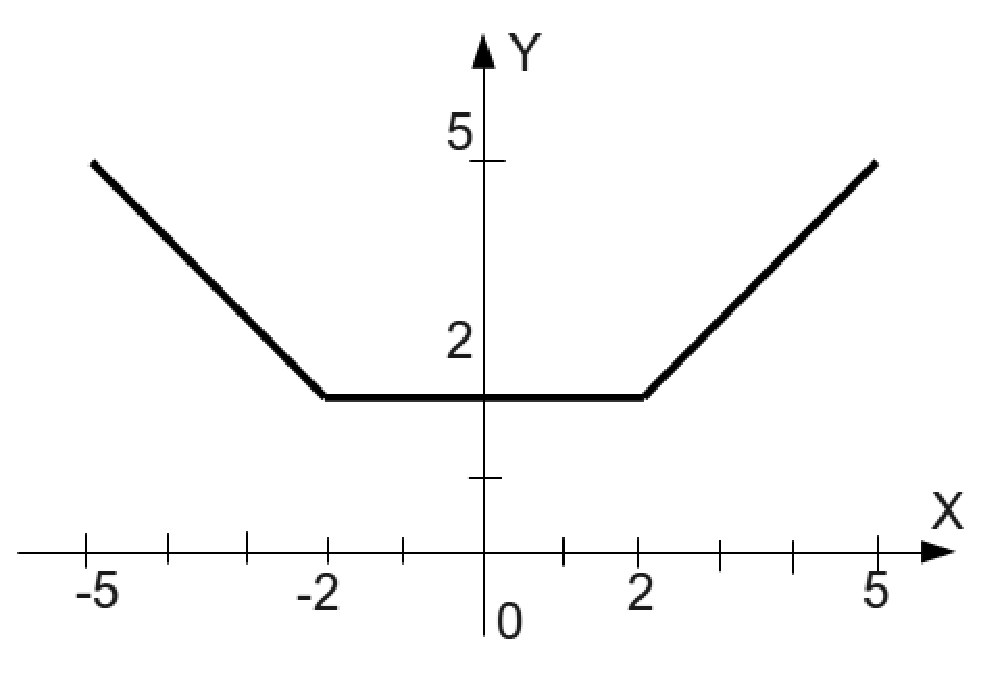
\includegraphics[width=0.32\textwidth,keepaspectratio]{img/ris_3_46}}
\ffigbox[\FBwidth]
{\caption{Задание~9}%
\label{ch03:refDrawing46}}
{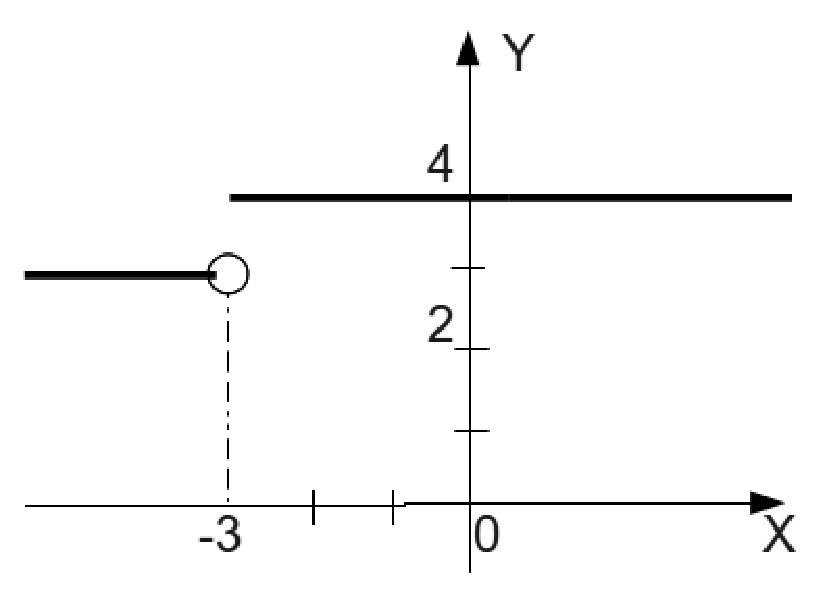
\includegraphics[width=0.32\textwidth,keepaspectratio]{img/ris_3_47}}
\end{floatrow}
\end{figure}%
%%%% end 45, 46, 47

%%%%%% рис 48, 49 и 50 в ряд 
\floatsetup[widefloat]{margins=hangleft}
\begin{figure}%
\begin{floatrow}[3]
\ffigbox[\FBwidth]
{\caption{Задание~10}%
\label{ch03:refDrawing47}}
{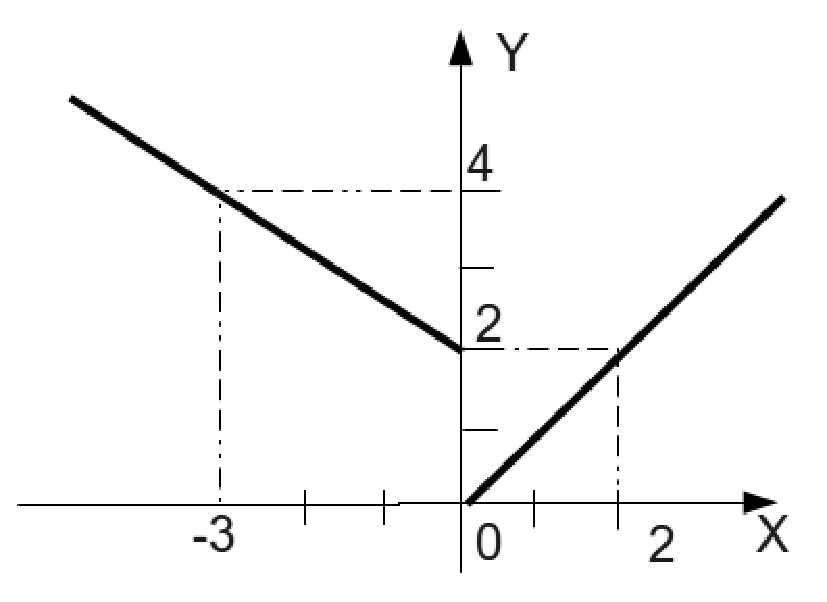
\includegraphics[width=0.32\textwidth,keepaspectratio]{img/ris_3_48}}
\ffigbox[\FBwidth]
{\caption{Задание~11}%
\label{ch03:refDrawing48}}
{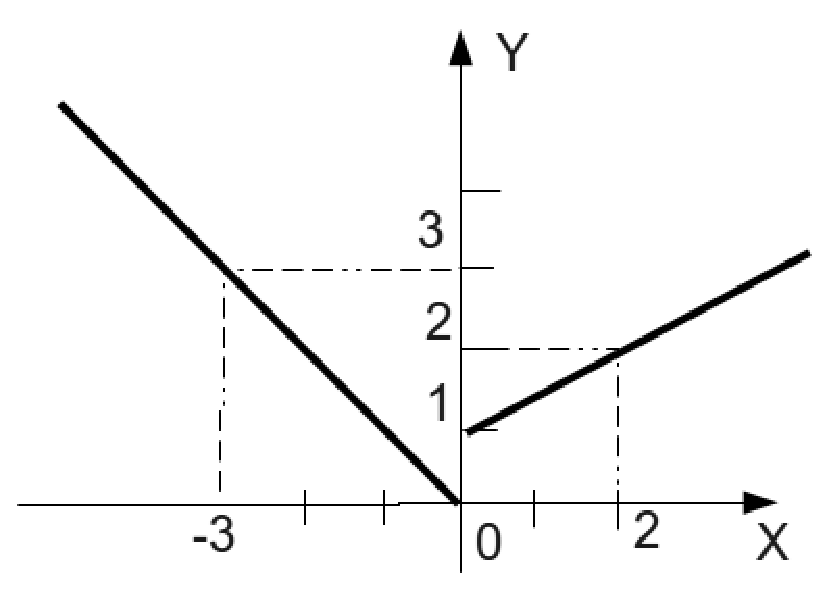
\includegraphics[width=0.32\textwidth,keepaspectratio]{img/ris_3_49}}
\ffigbox[\FBwidth]
{\caption{Задание~12}%
\label{ch03:refDrawing49}}
{\includegraphics[width=0.32\textwidth,keepaspectratio]{img/ris_3_50}}
\end{floatrow}
\end{figure}%
%%%% end 48, 49, 50

%%%%%% рис 51, 52 и 53 в ряд 
\floatsetup[widefloat]{margins=hangleft}
\begin{figure}%
\begin{floatrow}[3]
\ffigbox[\FBwidth]
{\caption{Задание~13}%
\label{ch03:refDrawing50}}
{\includegraphics[width=0.32\textwidth,keepaspectratio]{img/ris_3_51}}
\ffigbox[\FBwidth]
{\caption{Задание~14}%
\label{ch03:refDrawing51}}
{\includegraphics[width=0.32\textwidth,keepaspectratio]{img/ris_3_52}}
\ffigbox[\FBwidth]
{\caption{Задание~15}%
\label{ch03:refDrawing52}}
{\includegraphics[width=0.32\textwidth,keepaspectratio]{img/ris_3_53}}
\end{floatrow}
\end{figure}%
%%%% end 51, 52, 53

%%%%%% рис 54, 55 и 56 в ряд 
\floatsetup[widefloat]{margins=hangleft}
\begin{figure}%
\begin{floatrow}[3]
\ffigbox[\FBwidth]
{\caption{Задание~16}%
\label{ch03:refDrawing53}}
{\includegraphics[width=0.32\textwidth,keepaspectratio]{img/ris_3_54}}
\ffigbox[\FBwidth]
{\caption{Задание~17}%
\label{ch03:refDrawing54}}
{\includegraphics[width=0.32\textwidth,keepaspectratio]{img/ris_3_55}}
\ffigbox[\FBwidth]
{\caption{Задание~18}%
\label{ch03:refDrawing55}}
{\includegraphics[width=0.32\textwidth,keepaspectratio]{img/ris_3_56}}
\end{floatrow}
\end{figure}%
%%%% end 54, 55, 56

%%%%%% рис 57, 58 и 59 в ряд 
\floatsetup[widefloat]{margins=hangleft}
\begin{figure}%
\begin{floatrow}[3]
\ffigbox[\FBwidth]
{\caption{Задание~19}%
\label{ch03:refDrawing56}}
{\includegraphics[width=0.32\textwidth,keepaspectratio]{img/ris_3_57}}
\ffigbox[\FBwidth]
{\caption{Задание~20}%
\label{ch03:refDrawing57}}
{\includegraphics[width=0.32\textwidth,keepaspectratio]{img/ris_3_58}}
\ffigbox[\FBwidth]
{\caption{Задание~21}%
\label{ch03:refDrawing58}}
{\includegraphics[width=0.32\textwidth,keepaspectratio]{img/ris_3_59}}
\end{floatrow}
\end{figure}%
%%%% end 57, 58, 59

%%%% рис 60 и 61 бок о бок
\begin{figure}[h]
\begin{floatrow}
\floatbox{figure}[.35\textwidth][\FBheight][t]
{\caption{Задание~22}
\label{ch03:refDrawing59}}
{\includegraphics[width=0.32\textwidth,keepaspectratio]{img/ris_3_60}}%\hspace*{0.05\textwidth}
%
\floatbox{figure}[.35\textwidth][\FBheight][b]
{\caption{Задание~23}
\label{ch03:refDrawing60}}
{\includegraphics[width=0.32\textwidth]{img/ris_3_61}}
\end{floatrow}
\end{figure}

%%%% рис 62 и 63 бок о бок
\begin{figure}[h]
\begin{floatrow}
\floatbox{figure}[.35\textwidth][\FBheight][t]
{\caption{Задание~24}
\label{ch03:refDrawing61}}
{\includegraphics[width=0.32\textwidth,keepaspectratio]{img/ris_3_62}}%\hspace*{0.05\textwidth}
%
\floatbox{figure}[.35\textwidth][\FBheight][b]
{\caption{Задание~25}
\label{ch03:refDrawing62}}
{\includegraphics[width=0.32\textwidth]{img/ris_3_63}}
\end{floatrow}
\end{figure}

\subsection[Разветвляющийся процесс. Попадание точки в область на плоскости]{Разветвляющийся процесс. Попадание точки в
область на плоскости}
Разработать программу на языке \Sys{С++}. Даны вещественные числа $x$ и $y$. Определить,
принадлежит ли точка с координатами ($x$; $y$) заштрихованной области.
Варианты заданий представлены на рис.~\ref{ch03:refDrawing63}--\ref{ch03:refDrawing87}.


%%%%%% рис 64, 65 и 66 в ряд 
\floatsetup[widefloat]{margins=hangleft}
\begin{figure}[h]%
\begin{floatrow}[3]
\ffigbox[\FBwidth]
{\caption{Задание~1}%
\label{ch03:refDrawing63}}
{\includegraphics[width=0.32\textwidth,keepaspectratio]{img/ris_3_64}}
\ffigbox[\FBwidth]
{\caption{Задание~2}%
\label{ch03:refDrawing64}}
{\includegraphics[width=0.32\textwidth,keepaspectratio]{img/ris_3_65}}
\ffigbox[\FBwidth]
{\caption{Задание~3}%
\label{ch03:refDrawing65}}
{\includegraphics[width=0.32\textwidth,keepaspectratio]{img/ris_3_66}}
\end{floatrow}
\end{figure}%
%%%% end 64, 65, 66

%%%%%% рис 67, 68 и 69 в ряд 
\floatsetup[widefloat]{margins=hangleft}
\begin{figure}[h]%
\begin{floatrow}[3]
\ffigbox[\FBwidth]
{\caption{Задание~4}%
\label{ch03:refDrawing66}}
{\includegraphics[width=0.32\textwidth,keepaspectratio]{img/ris_3_67}}
\ffigbox[\FBwidth]
{\caption{Задание~5}%
\label{ch03:refDrawing67}}
{\includegraphics[width=0.32\textwidth,keepaspectratio]{img/ris_3_68}}
\ffigbox[\FBwidth]
{\caption{Задание~6}%
\label{ch03:refDrawing68}}
{\includegraphics[width=0.32\textwidth,keepaspectratio]{img/ris_3_69}}
\end{floatrow}
\end{figure}%
%%%% end 67, 68, 69

%%%%%% рис 70, 71 и 72 в ряд 
\floatsetup[widefloat]{margins=hangleft}
\begin{figure}[h]%
\begin{floatrow}[3]
\ffigbox[\FBwidth]
{\caption{Задание~7}%
\label{ch03:refDrawing69}}
{\includegraphics[width=0.32\textwidth,keepaspectratio]{img/ris_3_70}}
\ffigbox[\FBwidth]
{\caption{Задание~8}%
\label{ch03:refDrawing70}}
{\includegraphics[width=0.32\textwidth,keepaspectratio]{img/ris_3_71}}
\ffigbox[\FBwidth]
{\caption{Задание~9}%
\label{ch03:refDrawing71}}
{\includegraphics[width=0.32\textwidth,keepaspectratio]{img/ris_3_72}}
\end{floatrow}
\end{figure}%
%%%% end 70, 71, 72

%%%%%% рис 73, 74 и 75 в ряд 
\floatsetup[widefloat]{margins=hangleft}
\begin{figure}[h]%
\begin{floatrow}[3]
\ffigbox[\FBwidth]
{\caption{Задание~10}%
\label{ch03:refDrawing72}}
{\includegraphics[width=0.32\textwidth,keepaspectratio]{img/ris_3_73}}
\ffigbox[\FBwidth]
{\caption{Задание~11}%
\label{ch03:refDrawing73}}
{\includegraphics[width=0.32\textwidth,keepaspectratio]{img/ris_3_74}}
\ffigbox[\FBwidth]
{\caption{Задание~12}%
\label{ch03:refDrawing74}}
{\includegraphics[width=0.32\textwidth,keepaspectratio]{img/ris_3_75}}
\end{floatrow}
\end{figure}%
%%%% end 73, 74, 75

%%%%%% рис 76, 77 и 78 в ряд 
\floatsetup[widefloat]{margins=hangleft}
\begin{figure}[h]%
\begin{floatrow}[3]
\ffigbox[\FBwidth]
{\caption{Задание~13}%
\label{ch03:refDrawing75}}
{\includegraphics[width=0.32\textwidth,keepaspectratio]{img/ris_3_76}}
\ffigbox[\FBwidth]
{\caption{Задание~14}%
\label{ch03:refDrawing76}}
{\includegraphics[width=0.32\textwidth,keepaspectratio]{img/ris_3_77}}
\ffigbox[\FBwidth]
{\caption{Задание~15}%
\label{ch03:refDrawing77}}
{\includegraphics[width=0.32\textwidth,keepaspectratio]{img/ris_3_78}}
\end{floatrow}
\end{figure}%
%%%% end 76, 77, 78

%%%%%% рис 79, 80 и 81 в ряд 
\floatsetup[widefloat]{margins=hangleft}
\begin{figure}[h]%
\begin{floatrow}[3]
\ffigbox[\FBwidth]
{\caption{Задание~16}%
\label{ch03:refDrawing78}}
{\includegraphics[width=0.30\textwidth,keepaspectratio]{img/ris_3_79}}
\ffigbox[\FBwidth]
{\caption{Задание~17}%
\label{ch03:refDrawing79}}
{\includegraphics[width=0.30\textwidth,keepaspectratio]{img/ris_3_80}}
\ffigbox[\FBwidth]
{\caption{Задание~18}%
\label{ch03:refDrawing80}}
{\includegraphics[width=0.30\textwidth,keepaspectratio]{img/ris_3_81}}
\end{floatrow}
\end{figure}%
%%%% end 79, 80, 81

%%%%%% рис 82, 83 и 84 в ряд 
\floatsetup[widefloat]{margins=hangleft}
\begin{figure}[h]%
\begin{floatrow}[3]
\ffigbox[\FBwidth]
{\caption{Задание~19}%
\label{ch03:refDrawing81}}
{\includegraphics[width=0.30\textwidth,keepaspectratio]{img/ris_3_82}}
\ffigbox[\FBwidth]
{\caption{Задание~20}%
\label{ch03:refDrawing82}}
{\includegraphics[width=0.26\textwidth,keepaspectratio]{img/ris_3_83}}
\ffigbox[\FBwidth]
{\caption{Задание~21}%
\label{ch03:refDrawing83}}
{\includegraphics[width=0.30\textwidth,keepaspectratio]{img/ris_3_84}}
\end{floatrow}
\end{figure}%
%%%% end 82, 83, 84

%%%% рис 85 и 86 бок о бок
\begin{figure}[h]
\begin{floatrow}
\floatbox{figure}[.35\textwidth][\FBheight][t]
{\caption{Задание~22}
\label{ch03:refDrawing84}}
{\includegraphics[width=0.32\textwidth,keepaspectratio]{img/ris_3_85}}%\hspace*{0.05\textwidth}
%
\floatbox{figure}[.35\textwidth][\FBheight][b]
{\caption{Задание~23}
\label{ch03:refDrawing85}}
{\includegraphics[width=0.28\textwidth]{img/ris_3_86}}
\end{floatrow}
\end{figure}

%%%% рис 87 и 88 бок о бок
\begin{figure}[h]
\begin{floatrow}
\floatbox{figure}[.35\textwidth][\FBheight][t]
{\caption{Задание~24}
\label{ch03:refDrawing86}}
{\includegraphics[width=0.28\textwidth,keepaspectratio]{img/ris_3_87}}%\hspace*{0.05\textwidth}
%
\floatbox{figure}[.35\textwidth][\FBheight][b]
{\caption{Задание~25}
\label{ch03:refDrawing87}}
{\includegraphics[width=0.28\textwidth]{img/ris_3_88}}
\end{floatrow}
\end{figure}


\subsection[Разветвляющийся процесс. Пересечение линий и решение уравнений.]{Разветвляющийся процесс. Пересечение
линий и решение уравнений.}
Разработать программу на языке \Sys{С++} для следующих заданий:

\begin{enumerate}
\item Задан круг с центром в точке $O(x_0, y_0)$, радиусом $R_0$ и точка $A(x_1,y_1)$. 
Определить, находится ли точка внутри круга.
\item Задана окружность с центром в точке $O(x_0,y_0)$ и радиусом $R_0$. Определить, пересекается ли
заданная окружность с осью абсцисс, если пересекается --- найти точки пересечения.
\item Задана окружность с центром в точке $O(x_0,y_0)$ и радиусом $R_0$. Определить, пересекается ли
заданная окружность с осью ординат, если пересекается --- найти точки пересечения.
\item Задана окружность с центром в точке $O(0,0)$ и радиусом $R_0$ и
прямая $y=ax+b$. Определить, пересекаются ли прямая и
окружность. Если пересекаются, найти точки пересечения.
\item Заданы окружности. Первая с центром в точке $O(x_1,y_1)$ и радиусом
$R_1$, вторая с центром в точке $O(x_2,y_2)$ и радиусом
$R_2$. Определить, пересекаются окружности, касаются или не пересекаются.
\item Заданы три точки
$A(x_1,y_1)$, $B(x_2,y_2)$,$C(x_3,y_3)$. Определить, какая
из точек наиболее удалена от начала координат.
\item Заданы три точки $A(x_1,y_1)$, $B(x_2,y_2)$, $C(x_3,y_3)$. Определить, какая
из точек $B$ или $C$ наименее удалена от точки $A$.
\item Определить, пересекаются ли линии $y=ax+b$ и
$y=kx+m$. Если пересекаются, найти точку пересечения.
\item Определить, пересекает ли линия $y=ax+b$ ось абсцисс. Если пересекает, найти точку пересечения.
\item Определить, пересекаются ли линии
$y=ax^3+bx^2+cx+d$ и $y=kx+m$. Если пересекаются, найти точки пересечения.
\item Определить, пересекаются ли линии
$y=ax^3+bx^2+cx+d$
и
$y=kx^3+mx^2+nx+p$.
Если пересекаются, найти точки пересечения.
\item Определить, пересекаются ли линии
$y=ax^3+bx^2+cx+d$
и
$y=ax^3+mx^2+nx+p$.
Если пересекаются, найти точки пересечения.
\item Определить, пересекаются ли линии
$y=ax^3+bx^2+cx+d$
и $y=mx^2+nx+p$. Если
пересекаются, найти точку пересечения.
\item Определить, пересекает ли линия
$y=ax^3+bx^2+cx+d$
ось абсцисс. Если пересекает, найти точку пересечения.
\item Определить, пересекаются ли параболы
$y=ax^2+bx+c$ и $y=dx^2+mx+n$. Если
пересекаются, то найти точки пересечения.
\item Определить, пересекаются ли линии
$y=bx^2+cx+d$ и
$y=kx+m$. Если пересекаются, найти точки пересечения
\item Найти точки пересечения линии
$y=ax^2+bx+c$ с осью
абсцисс. Если линии не пересекаются выдать соответствующее сообщение.
\item Определить, пересекаются ли линии
$y=ax^4+bx^3+cx^2+dx+f$
и
$y=bx^3+mx^2+dx+p$.
Если пересекаются, найти точки пересечения.
\item Определить, пересекаются ли линии
$y=ax^4+bx^2+kx+c$
и
$y=mx^2+kx+p$.
Если пересекаются, найти точки пересечения.
\item Определить, пересекает ли линия
$y=ax^4+bx^2+c$
ось абсцисс. Если пересекает, найти точки пересечения.
\item Найти комплексные корни уравнения
$y=ax^4+bx^2+c$.
Если в уравнении нет комплексных корней, вывести соответствующее сообщение.
\item Найти комплексные корни уравнения
$y=ax^3+bx^2+cx+d$. Если в
уравнении нет комплексных корней, вывести соответствующее сообщение.
\item Найти комплексные корни уравнения $y=ax^2+bx+c$. Если в
уравнении нет комплексных корней, вывести соответствующее сообщение.
\item Заданы точки $A(x_1,y_1,z_1)$ и $B(x_2,y_2,z_2)$. Определить, какая из точек наименее удалена от начала координат.
\item Даны координаты точки, не лежащей на координатных осях $OX$ и $OY$. Определить номер координатной четверти, в которой
находится данная точка.
\end{enumerate}

\subsection[Циклический процесс. Вычисление значений функции]{Циклический процесс. Вычисление значений функции}

Разработать программу на языке \Sys{С++}. Для решения задачи использовать операторы \Sys{for},
\Sys{while}, \Sys{do}. Варианты заданий:

\begin{enumerate}
\item Вывести на экран таблицу значений функции синус в диапазоне от  $-2\cdot \pi $ до  $2\cdot \pi $  с шагом~
$\frac{\pi}{8}$.
\item Вывести на экран таблицу квадратов первых десяти целых положительных чисел.
\item Вывести на экран таблицу значений функции косинус в диапазоне от  $-2\cdot \pi $  до  $2\cdot \pi $  с шагом~
$\frac{\pi}{8}$.
\item Вывести на экран таблицу кубов первых десяти целых положительных чисел.
\item Вывести на экран таблицу значений квадратов синусов в диапазоне от  $-\pi$  до  $\pi$  с шагом~$\frac{\pi}{12}$.
\item Вывести на экран таблицу значений квадратов косинусов в диапазоне от 0 до $2\cdot \pi$ с шагом~$\frac{\pi}{10}$.
\item Вывести на экран таблицу квадратов первых десяти целых чётных положительных чисел.
\item Вывести на экран таблицу квадратов первых десяти целых нечётных положительных чисел.
\item Вывести на экран таблицу значений удвоенных синусов в диапазоне от $-a$ до $a$ с шагом $h$. Значения $a$ и
 $h$  вводятся с клавиатуры.
\item Вывести на экран таблицу значений удвоенных косинусов в диапазоне от  $a$  до  $b$  с шагом  $h$. Значения  $a$,
 $b$  и  $h$  вводятся с клавиатуры.
\item Вывести на экран таблицу кубов первых десяти целых нечётных положительных чисел.
\item Вывести на экран таблицу кубов первых десяти целых чётных положительных чисел.
\item Вывести на экран таблицу значений функции  $y=e^{2x}$ в диапазоне от  $-a$  до  $a$  с шагом  $h$. Значения  $a$ 
и  $h$  вводятся с клавиатуры.
\item Вывести на экран таблицу значений функции  $y=5\cdot e^{-3x}$  в диапазоне от  $a$  до  $b$  с шагом~$h$.
Значения  $a$,  $b$  и  $h$  вводятся с клавиатуры.
\item Вывести на экран таблицу квадратов первых десяти целых отрицательных чисел.
\item Вывести на экран таблицу кубов первых десяти целых отрицательных чисел.
\item Вывести на экран таблицу квадратных корней первых десяти целых положительных чисел.
\item Вывести на экран таблицу кубических корней первых десяти целых положительных чисел.
\item Вывести на экран таблицу значений функции  $y=2\cdot x^2+3\cdot x-1$  в диапазоне от  $-a$  до  $a$  с шагом~
$h$. Значения  $a$  и  $h$  вводятся с клавиатуры.
\item Вывести на экран таблицу значений функции  $y=5.4\cdot x^{3}-2.8\cdot x^{2}-x+1.6$  в диапазоне от  $a$  до  $b$ 
с шагом  $h$. Значения  $a$,  $b$  и  $h$  вводятся с клавиатуры.
\item Вывести на экран таблицу квадратных корней первых десяти целых положительных чётных чисел.
\item Вывести на экран таблицу квадратных корней первых десяти целых положительных нечётных чисел.
\item Вывести на экран таблицу значений функции  $y=-1.8\cdot x^3-e^2x+\frac{1}{6}$  в диапазоне от  $-3$ до  $4$  с
шагом~$\frac{1}{2}$.
\item Вывести на экран таблицу значений функции  $y=-1.3\cdot x^2-\frac{e^x}{4}$  в диапазоне от  $-2$  до  $2$  с
шагом~$\frac{1}{4}$.
\item Вывести на экран таблицу степеней двойки в диапазоне от  0  до  10  с шагом~1.
\end{enumerate}

\subsection[Циклический процесс. Последовательности натуральных чисел]{Циклический процесс. Последовательности
натуральных чисел}
Разработать программу на языке \Sys{С++} для следующих заданий:

\begin{enumerate}
\item Дано целое положительное число $N$. Вычислить сумму натуральных нечётных чисел не превышающих
это число.
\item Дано целое положительное число $N$. Вычислить произведение натуральных чётных чисел не
превышающих это число.
\item Дано целое положительное число $N$. Вычислить количество натуральных чисел кратных трём и не
превышающих число~$N$.
\item Задано целое положительное число $n$. Определить значение выражения:
 $\displaystyle P=\frac{n!}{\sum\limits_{i=1}^{n}i}.$
\item Вычислить количество натуральных двузначных чётных чисел не делящихся на~10.
\item Задано целое положительное число $n$. Определить значение выражения:
$\displaystyle P=\frac{\sum\limits_{i=1}^ni^2}{n!}.$
\item Вычислить сумму натуральных удвоенных чисел не превышающих~25.
\item Задано целое положительное число $n$. Определить значение выражения:
$P=\frac{\sum\limits_{i=3}^{n}i-2}{(n+1)!}.$
\item Дано целое положительное число $N$. Вычислить сумму квадратов натуральных чётных чисел не
превышающих это число.
\item Дано целое положительное число $N$. Вычислить количество натуральных чисел кратных пяти и не
превышающих число $N$.
\item Определить значение выражения:
 $P=\frac{\sum\limits_{i=0}^{5}3^{i}}{5!}.$
\item Дано целое положительное число $N$. Вычислить сумму удвоенных натуральных нечётных чисел не
превышающих это число.
\item Задано целое положительное число $n$. Определить значение выражения:
 $P=\sum\limits_{i=2}^{n}i^{2}-i.$
\item Найти сумму нечётных степеней двойки. Значение степени изменяется от 1 до~9.
\item Задано целое положительное число $n$. Определить значение выражения:
 $P=\frac{1}{3}\cdot {\sum\limits_{i=1}^{n}2\cdot i^{2}-i+1}.$
\item Дано целое положительное число $N$. Вычислить произведение натуральных чисел кратных трём и не
превышающих число~$N$.
\item Задано целое положительное число $n$. Определить значение выражения:
 $P=\sum\limits_{i=3}^{n+2}2\cdot i-4.$
\item Вычислить сумму натуральных трёхзначных чисел кратных пяти и не делящихся на десять.
\item Определить значение выражения:
 $P=\sum\limits_{i=0}^{10}2^{i}.$
\item Вычислить количество натуральных двузначных нечётных чисел не делящихся на~5.
\item Задано целое положительное число $n$. Определить значение выражения:
 $P=\frac{\sum\limits_{i=0}^{n-1}i+1}{(2n)!}.$
\item Задано целое положительное число $n$. Определить значение выражения:
 $P=\frac{\sum\limits_{i=5}^{15}i}{(2\cdot n+1)!}.$
\item Найти произведение чётных степеней двойки. Значение степени изменяется от 0 до~8.
\item Вычислить произведение натуральных чисел не превышающих~15.
\item Вычислить произведение натуральных двузначных чисел кратных трём и не делящихся на~10.
\end{enumerate}

\subsection[Циклический процесс. Последовательности произвольных чисел]{Циклический процесс. Последовательности
произвольных чисел}
Разработать программу на языке \Sys{С++} для следующих заданий:

\begin{enumerate}
\item Вводится последовательность ненулевых чисел, 0 --- конец последовательности. Определить сумму положительных
элементов последовательности.
\item Вычислить сумму отрицательных элементов последовательности из $N$ произвольных чисел.
\item Вводится последовательность ненулевых чисел, 0 --- конец последовательности. Определить, сколько раз
последовательность поменяет знак.
\item В последовательности из $N$ произвольных чисел подсчитать количество нулей.
\item Вводится последовательность ненулевых чисел, 0 --- конец последовательности. Определить наибольшее число в
последовательности.
\item Вводится последовательность из $N$ произвольных чисел найти наименьшее число в
последовательности.
\item Вводится последовательность ненулевых чисел, 0 --- конец последовательности. Определить среднее значение элементов
последовательности.
\item Вводится последовательность из $N$ произвольных чисел, найти среднее значение положительных
элементов последовательности.
\item Вводится последовательность ненулевых чисел, 0 --- конец последовательности. Подсчитать процент положительных и
отрицательных чисел.
\item Вводится последовательность из $N$ произвольных чисел. Определить процент положительных,
отрицательных и нулевых элементов. 
\item Вводится последовательность из $N$ произвольных чисел. Вычислить разность между наименьшим и
наибольшим значениями последовательности.
\item Вводится последовательность из $N$ положительных целых чисел. Найти наименьшее число среди
чётных элементов последовательности.
\item Вводится последовательность из $N$ целых чисел. Определить, является ли эта
последовательность знакочередующейся.
\item Определить, является ли последовательность из $N$ произвольных чисел строго возрастающей (каждый
следующий элемент больше предыдущего).
\item Вводится последовательность произвольных чисел, 0 --- конец последовательности. Определить, является ли эта
последовательность строго убывающей (каждый следующий элемент меньше предыдущего).
\item Вводится последовательность ненулевых целых чисел, 0 --- конец последовательности. Определить среднее значение
чётных элементов последовательности.
\item Вводится последовательность из $N$ произвольных чисел, найти среднее значение отрицательных
элементов последовательности.
\item В последовательности из $N$ целых чисел подсчитать количество чётных и нечётных чисел.
\item Вводится последовательность целых чисел, 0 --- конец последовательности. Определить процент чётных и нечётных чисел
в последовательности.
\item Вводится последовательность из $N$ целых чисел. Определить, содержит ли последовательность хотя
бы два соседних одинаковых числа.
\item Вводится последовательность целых чисел, 0 --- конец последовательности. Определить наибольшее число среди нечётных
элементов последовательности.
\item Вводится последовательность произвольных чисел, 0 --- конец последовательности. Определить сумму и количество чисел
в последовательности.
\item Вводится последовательность из $N$ произвольных чисел. Найти сумму положительных и сумму
отрицательных элементов последовательности.
\item Вводится последовательность произвольных чисел, 0 --- конец последовательности. Определить отношение минимального и
максимального элементов друг к другу.
\item Вводится последовательность из $N$ целых чисел. Определить количество одинаковых рядом стоящих
чисел.
\end{enumerate}

\subsection[Циклический процесс. Работа с цифрами в числе]{Циклический процесс. Работа с цифрами в числе}
Разработать программу на языке \Sys{С++} для следующих заданий:

\begin{enumerate}
\item Определить, является ли целое положительное число \emph{совершённым}. Совершённое число равно сумме
всех своих делителей, не превосходящих это число. Например, 6=1+2+3 или 28=1+2+4+7+14.
\item Проверить, является ли пара целых положительных чисел \emph{дружественными}. Два различных натуральных
числа являются дружественными, если сумма всех делителей первого числа (кроме самого числа) равна второму числу.
Например, 220 и 284, 1184 и 1210, 2620 и 2924, 5020 и 5564.
\item Определить, является ли целое положительное число \emph{недостаточным}. Недостаточное число всегда
больше суммы всех своих делителей за исключением самого числа.
\item Вводится целое положительное число. Определить количество чётных и нечётных цифр в числе.
\item Вводится целое положительное число. Найти число, которое равно сумме кубов цифр исходного числа.
\item Вводится целое положительное число. Определить, совпадает ли сумма цифр, 
расположенных до середины числа, с суммой цифр расположенных после. Например, задано число из восьми 
цифр 12112021. Здесь, сумма первых четырёх цифр, равна сумме следующих четырёх цифр $1+2+1+1=2+0+2+1=5$. 
Или, задано число из семи цифр 3456444, тогда $3+4+5=4+4+4=12$. Здесь цифра 6 не учитывается.
\item Вводится целое положительное число. Найти суммы чётных и нечётных цифр заданного числа.
\item Задано целое положительное число. Определить количество его чётных и нечётных делителей.
\item Проверить, являются ли два целых положительных числа \emph{взаимно простыми}. Два различных
натуральных числа являются взаимно простыми, если их наибольший общий делитель равен единице.
\item Определить, является ли целое положительное число \emph{составным}. Составное число имеет более двух
делителей, то есть не является \emph{простым}.
\item Вводится целое положительное число. Найти наименьшую цифру числа.
\item Задано целое положительное число. Определить, является ли оно \emph{числом Армстронга}. Число
Армстронга --- натуральное число, которое равно сумме своих цифр, возведённых в степень, равную количеству его цифр.
Например, десятичное число 153 --- число Армстронга, потому что:  $1^3+3^3+5^3=1+27+125=153$.
\item Вводится целое положительное число. Найти произведение всех ненулевых цифр числа.
\item Вводится целое положительное число. Найти наибольшую цифру числа.
\item Вводится целое положительное число. Определить позицию наибольшей цифры в числе.
\item Вводится целое положительное число. Найти число, которое равно сумме удвоенных цифр исходного числа.
\item Вводится целое положительное число. Найти число, которое равно сумме квадратов цифр исходного числа.
\item Задано целое положительное число. Определить сумму его делителей.
\item Вводится целое положительное число. Определить позицию наименьшей цифры в числе.
\item Проверить, что два целых положительных числа не являются \emph{взаимно простыми}. Различные
натуральные числа не являются взаимно простыми, если их наибольший общий делитель отличен от единицы.
\item Убедиться, что заданное целое положительное число не является \emph{палиндромом}. Числа-палиндромы
симметричны относительно своей середины, например, 12021 или 454.
\item Убедиться, что заданное целое положительное число не является \emph{совершённым}. Совершённое число
равно сумме всех своих делителей, не превосходящих это число. Например, 6=1+2+3 или 28=1+2+4+7+14.
\item Проверить, что два целых положительных числа не являются \emph{дружественными}. Два различных
натуральных числа являются дружественными, если сумма всех делителей первого числа (кроме самого числа) равна второму
числу. Например, 220 и 284, 1184 и 1210, 2620 и 2924, 5020 и 5564.
\item Вводится целое положительное число. Найти число, которое равно сумме утроенных цифр исходного числа.
\item Вводятся два целых положительных числа. Найти сумму их цифр. 
\end{enumerate}

\subsection[Вложенные циклы]{Вложенные циклы}
Разработать программу на языке \Sys{С++} для следующих заданий:

\begin{enumerate}
\item Дано натуральное число $P$. Вывести все простые числа не
превосходящие $P$.
\item Дано натуральное число $P$. Вывести все совершённые числа не превосходящие
$P$.
\item Вводится последовательность положительных целых чисел, 0 --- конец последовательности. Определить количество
совершённых чисел в последовательности.
\item Вводится последовательность положительных целых чисел, 0 --- конец последовательности. Определить количество простых
чисел в последовательности.
\item Вводится последовательность из $N$ положительных целых чисел. Для каждого элемента
последовательности вычислить факториал.
\item Вводится последовательность из $N$ положительных целых чисел. Вывести на экран все числа ---
палиндромы. Если таких чисел нет, выдать соответствующее сообщение.
\item Вводится последовательность из $N$ положительных целых чисел. Определить разрядность каждого
числа.
\item Вводится последовательность из $N$ положительных целых чисел. Вывести на экран количество
делителей каждого числа.
\item Вводится последовательность положительных целых чисел, 0 --- конец последовательности. Определить сумму цифр каждого
элемента последовательности.
\item Дано $K$ наборов ненулевых целых чисел. Признаком завершения каждого набора является число 0. Для каждого набора
вывести количество его элементов. Вычислить общее количество элементов.
\item Дано $K$ наборов ненулевых целых чисел. Признаком завершения каждого набора является число 0. Для каждого набора
вычислить среднее арифметическое его элементов.
\item Даны $K$ наборов целых чисел по $N$ элементов в каждом наборе. Для каждого набора найти наибольшее значение его
элементов.
\item Даны $K$ наборов целых чисел по $N$ элементов в каждом наборе. Определить, есть ли среди наборов данных
знакочередующиеся последовательности.
\item Даны $K$ наборов целых чисел по $N$ элементов в каждом наборе. Определить, есть ли среди наборов данных строго
возрастающие последовательности.
\item Дано $K$ наборов ненулевых целых чисел. Признаком завершения каждого набора является число 0. Для каждого набора
найти наименьшее значение его элементов.
\item Даны $K$ наборов целых чисел по $N$ элементов в каждом наборе. Для каждого набора вычислить произведение ненулевых
элементов.
\item Даны $K$ наборов целых чисел по $N$ элементов в каждом наборе. Найти наибольшее число для всех наборов.
\item Дано $K$ наборов ненулевых целых чисел. Признаком завершения каждого набора является число 0. Вычислить среднее
арифметическое всех элементов во всех наборах.
\item Дано $K$ наборов ненулевых целых чисел. Признаком завершения каждого набора является число 0. Найти количество
возрастающих наборов.
\item Дано $K$ наборов ненулевых целых чисел. Признаком завершения каждого набора является число 0. Найти количество
убывающих наборов.
\item Дано $K$ наборов ненулевых целых чисел. Признаком завершения каждого набора является число 0. Найти количество
наборов не являющихся знакочередующимися.
\item Дано $K$ наборов ненулевых целых чисел. Признаком завершения каждого набора является число 0. Найти количество
наборов элементы которых не возрастают и не убывают.
\item Даны целые положительные числа $N$ и $M$ ($N<M$). Вывести все целые числа от $N$ до $M$ включительно; при этом
каждое число должно выводиться столько раз, каково его значение (например, число 5 выводится 5 раз).
\item Дано целое число $N>0$. Найти сумму 1! + 2! + 3! + … + $N$!
\item Даны целые числа $N$ и $M$ ($N<M$). Вывести все целые числа от $N$ до $M$ включительно; при этом число $N$ должно
выводиться 1 раз, число $N + 1$ должно выводиться 2 раза и т. д.
\end{enumerate}
